\chapter*{Theory Introduction}
The ultimate goal of searches for DM particles and their interactions is to establish the correct theory of DM. If successful, this will likely reduce the updated version of the present review to an addition of an extra line in the expression for the  SM Lagrangian, as well as some accompanying discussion of the resulting phenomenology.

At present, however, we have only limited knowledge about DM, and no definitive experimental signal of its interactions. 
As a consequence, there is a proliferation of theoretical ideas about what DM could be.
In fact, in its essence DM is such a simple and general idea that 
proposing specific realizations may even be {\em too easy}. 
From the perspective of particle physics, it is reasonable to expect that DM will be described by a renormalizable relativistic Quantum Field Theory (QFT), a highly predictive approach that requires only the symmetries of the Lagrangian and the quantum numbers of the DM particle(s) to make predictions, using a limited set of parameters. 
The triumph of this approach is the Standard Model,
which enabled particle physicists to anticipate numerous experimental findings.
In parts of the DM research field, especially when focusing on cosmology or astrophysics, the bar for writing down theories of DM is lower, focusing on phenomenological consequences at hand and only hoping that the effective description fits into a QFT framework. 

This leaves us with a daunting task of reviewing the theories of DM, where on one hand we run the risk of producing a long useless list of possibilities, and on the other hand we may be leaving out the theoretical description of DM that turns out to be realized in Nature. In this endeavour, we will use the crutch that many theorists lean on when trying to compensate for the lack of experimental information about DM, and focus more heavily on speculations that are {\em theoretically well-motivated}.
The interpretation of what is {\em theoretically well-motivated} is subjective, but it usually implies one of the following:
\begin{enumerate}\label{criteriaDMth}
\item {\bf DM theories motivated by other issues}, such as 
the naturalness of the Higgs mass, the QCD $\theta$ problem,
the nature of dark energy, etc. 

\item {\bf Simple theories}, where this either denotes 
models that add the fewest additional degrees of freedom (a single scalar or fermion) or possess a minimal structure (one electroweak multiplet, a single new symmetry, only gravitational interactions, etc).
Note that sectors with complex phenomenology can sometimes follow from simple theories (an example is, for instance, the SU(3) strong interaction in the SM).

\item {\bf Predictive theories}, where DM properties are predicted in terms of 
a small number of free parameters, ideally zero.

\item {\bf Elegant theories},  which provide a plausible explanation for some of the
puzzling DM properties, such as: why is DM stable? Why is DM neutral? Why are the abundances of DM and visible matter comparable? 

\item {\bf Prototypical theories}.
Theories that employ ingredients that tend to appear, at least in some limit, in more complex theories.
For example DM as a supersymmetric wino can behave as any other fermionic electroweak triplet with zero hypercharge.

\item {\bf Theories that predict novel signals}, or at least lead to very distinct signals.  \label{DMTsignals}
\end{enumerate}
Fig.\fig{what} shows a map of some DM theories that score high on one or more of the above criteria, many of which we, at least briefly, review below. 


\stepcounter{chapter}
\begin{figure}[h]
$$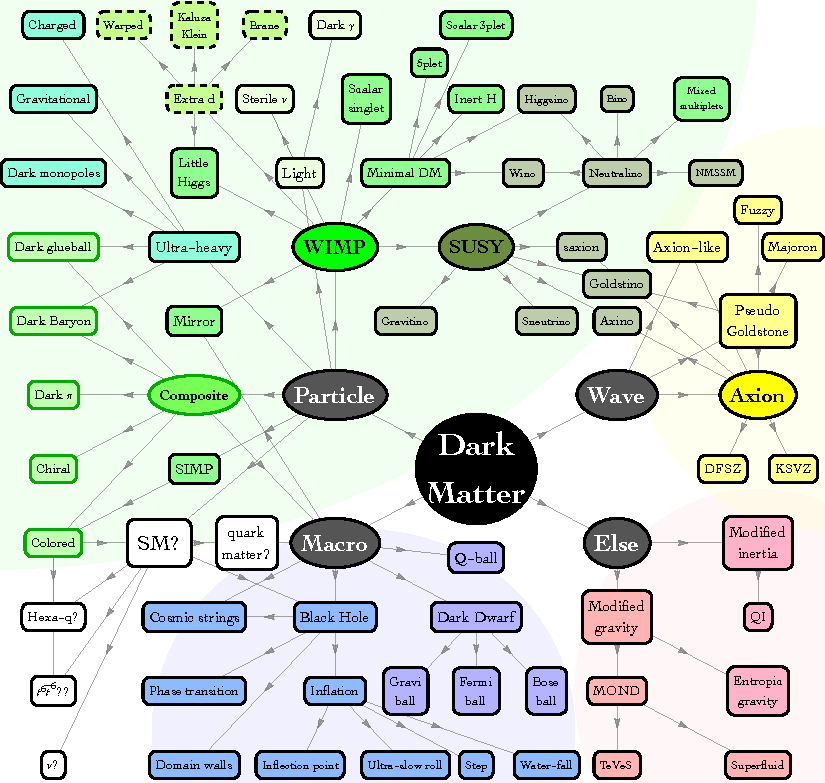
\includegraphics[width=\textwidth]{figs/DMtheoryMap}$$
\caption[Map of DM theories]{\em  \label{fig:what}  A map showcasing some of the main tentative DM theories.}
\end{figure}
\addtocounter{chapter}{-1}

\chapter{Theories of Dark Matter}
\label{models}
\stepcounter{figure}
In this chapter we present varios speculative theories of particle DM that primarily align with criteria 2 to 6 listed on page~\pageref{criteriaDMth}, i.e., the simple, predictive, elegant, prototypical and/or novel theories that are usually {\em not} motivated by external particle physics considerations. 
The subsequent chapter~\ref{BigDMtheories} will  focus instead on theories that mostly align with criterion 1, i.e.,~the theories motivated by `bigger' particle physics issues.


\smallskip

The chapter is organized, somewhat arbitrarily, as follows. 
In section~\ref{SMDM} we first summarize why the Standard Model fails to provide a good DM candidate.
We then explore DM candidates beyond the SM, using their SM interactions as an organizing principle.
First, we consider DM candidates that do not carry any SM charge: 
a scalar singlet (section \ref{ScalarSinglet}) or a fermionic singlet (section \ref{FermionSinglet}). 
Next, we move to DM candidates that are charged under the SM gauge group: 
DM might carry a small nonzero electric charge (section \ref{sec:ChargedDM}, with a more detailed discussion already given in~\ref{sec:milicharged}) or be charged under QCD (section~\ref{sec:ColoredDM}), while in section~\ref{sec:WIMPs} we discuss a class of DM particles that carry a weak charge (WIMPs) and its extensions. 
The Minimal Dark Matter candidates (section \ref{MDM}) are special cases within the WIMP category.
This is followed by a review of DM particles that are charged under hypothetical new forces or that interact with the SM via a `portal' (section \ref{sec:darksectors}).
The new forces can allow DM to be a composite particle, as discussed in section \ref{sec:compositeDM}. 
Dark sectors with a non-trivial group structure can produce DM that consists of dark monopoles, as we discuss in section \ref{Dmonopoles}.
Some dark sectors can generate a DM asymmetry analogous to the matter asymmetry, as discussed in section~\ref{sec:AsymmetricDMth}.
Finally, in section \ref{GravDM}, we consider the possibility that DM has no other interactions but the gravitational one.






\begin{table}[t]
$$\begin{array}{lcccccc}
\hbox{Fields}&{\rm spin} &{\rm U}(1)_Y&\SU(2)_L&\SU(3)_{\rm c}&L&B\cr \hline \rowcolor[rgb]{0.99,0.97,0.97}
U = u_R^c &1/2& -{2 \over 3} & 1 & \bar{3} &\phantom{-}0&-\frac13\cr \rowcolor[rgb]{0.99,0.97,0.97}
D = d_R^c &1/2& \phantom{-}{1 \over 3}& 1 &\bar{3} &\phantom{-}0&-\frac13\cr \rowcolor[rgb]{0.99,0.97,0.97}
Q=(u_L, d_L) &1/2 &\phantom{-} {1\over 6}  & 2 & 3&\phantom{-}0&\phantom{-}\frac13\cr \rowcolor[rgb]{0.95,0.97,0.97}
L=(\nu_L, e_L) &1/2& -{1 \over 2} & 2 &1&\phantom{-}1&\phantom{-}0\cr\rowcolor[rgb]{0.95,0.97,0.97}
E = e_R^c &1/2&\phantom{-}1 & 1 &1  &-1&\phantom{-}0\cr \rowcolor[rgb]{0.97,0.97,0.93}
H = (0,v+h/\sqrt{2})& 0&\phantom{-}{1 \over 2} & 2 &1&\phantom{-}0&\phantom{-}0\cr 
\end{array}$$
\caption[Standard Model]{\em List of {\bfseries Standard Model} Weyl fermions (quarks and leptons) and scalars, their charges under gauge interactions, and the
 lepton and baryon number accidental symmetries.\label{tab:SM}}
\end{table}





\section{Dark Matter in the Standard Model?}
\label{SMDM}
\index{Standard Model}
\index{DM theory!Standard Model}
Table~\ref{tab:SM} summarizes the particle content of the Standard Model (SM). Given this content, we 
first discuss why there is no dark matter candidate within the SM,
summarising the non-trivial attempts in this direction.
We first discuss elementary particles, moving then to bound composite states bound by
QCD, electroweak forces, nuclear forces, gravitational forces.

\subsection{Elementary: neutrino DM?}\label{neutrinoDM}
SM neutrinos are electrically neutral, weakly-interacting, stable particles, endowed with a non-zero mass: they pass most of the criteria discussed in section \ref{sec:DMparticle} for particle DM, and thus are at first sight a good candidate. 

In addition, neutrinos are very abundant in the Universe. According to  Big Bang cosmology, the SM neutrinos decouple while still relativistic, at the temperature
\beq 
T_\gamma=T_\nu\sim v^{4/3}/M_{\rm Pl}^{1/3}\sim \hbox{few MeV},
\eeq
where $v$ is the electroweak VEV. 
At this temperature, the neutrino interaction rate, $\Gamma_\nu \sim \sigma_{\nu e} n_e \sim T^5/v^4$, becomes smaller than 
the Hubble rate $H \sim T^2/M_{\rm Pl}$.
At neutrino decoupling the SM plasma consists mostly of $e^\pm$ and photons, so that the entropy density  is proportional to
$g_{*s} = 2+ 4(7/8) = 11/2$.
Later, when the temperature drops to $T_\gamma\sim m_e$ the electrons annihilate with positrons, heating $\gamma$ but not $\nu$,
while $g_{*s}$ decreases to $g_{*s}=2$ (plasma is now composed only of $\gamma$).
Since $Y_\nu = n_\nu/s $ stays constant, the neutrinos now have a lower temperature then photons, $T_\nu =T_\gamma (4/11)^{1/3}$.
This means that the number densities are related, $n_\nu/n_\gamma = 3/11$
where $n_\nu$ is the number density for a single generation of neutrinos and antineutrinos.
These cosmic background neutrinos have not yet been directly observed.


Neutrinos with mass $m_\nu \gg T_\nu$ contribute to the cosmological
energy density as
\beq
\label{eq:rhonu}
\rho_\nu = \sum_\nu m_\nu n_\nu, \quad {\rm or \ equivalently \ as} \quad \Omega_\nu h^2 = \frac{\sum_\nu m_\nu}{94 \ {\rm eV}},
\eeq
where for the latter equation we have used the standard definitions, see Appendix \ref{app:Cosmology}. Here, the sum runs over the 3 generations. The cosmological DM density would then be reproduced if $\sum_\nu  m_\nu \approx 11\eV$.

\medskip

However, the possibility of neutrinos being all of DM is excluded for several reasons.
First of all, DM composed of neutrinos with $11\eV$ mass would behave as warm dark matter, conflicting with the bounds in section~\ref{sec:WarmDM}.
Actually neutrinos must be lighter, $m_\nu \circa{<}\eV$, 
as dictated by laboratory bounds on beta-decay spectra and (if neutrinos are Majorana) on neutrino-less double beta decay~\cite{NuOsc,mnu_KATRIN}.
This means that ordinary neutrinos cannot be all of the DM, and that neutrinos in cosmology must be a (hot) component with an abundance well below the DM abundance.
Then bounds from matter clustering in cosmology and from the CMB imply $\sum_\nu m_\nu \circa{<}\hbox{few}\ 0.1\eV$, with the precise value depending on the assumed cosmological model and the employed dataset~\cite{mnu_cosmo}. 


In summary, SM neutrinos cannot be DM because: 1) their weak interactions imply a nearly thermal abundance; 2) they are too light.
Hypothetical extra `{\em sterile neutrinos}' can be heavier and don't have weak interactions: 
sterile neutrinos can be Dark Matter candidates, as will be discussed in section~\ref{FermionSinglet}.



\subsection{QCD bound states: quark matter?} 
\label{sec:quarkmatter}
\index{Quark matter}
\index{Nuggets!quark}
Next, let's explore the possibility that exotic bound states of quarks could be the DM.
Several authors, mostly around 1984, proposed that DM could consist of macroscopic objects, known as \index{Strangelets}\index{Quark nuggets} \index{Nuclearities} `{\bf quark nuggets}' (also called `{\bf strangelets}' or `{\bf nuclearites}'\footnote{Sometimes these terms are used  to distinguish objects of different sizes and masses within the category of `quark matter' objects. However, since this distinction does not seem to be consistently used in the literature, we will treat the three terms as synonymous.})~\cite{quark:matter:DM}.
Quark nuggets would consist of a very large number of bound quarks, with approximately equal abundances of $u$, $d$, and $s$ quarks. They would be denser than normal nuclear matter, since the presence of three flavors of quarks, in contrast to the two quark flavors in normal matter, allows for a higher density that is still compatible with the Pauli exclusion principle. They would have a very large baryon number (above $10^2$ and possibly up to about $10^{57}$), a mass ranging from $10^{-8}$ kg to $10^{20}$ kg and a size from femtometers to meters. 
In a first approximation they would have zero electric charge, since the charges of the $u,d,$ and $s$ quarks cancel each other out. However, because of the non-zero quark masses, the cancellation is not perfect. In particular, given their larger mass, the $s$ quarks are slightly less abundant hence strangelets typically have a net charge which is positive. This is welcome news, because negatively charged strangelets would have devastating consequences, eating up the nuclei they would encounter, while positively charged ones are electrostatically repelled by nuclei. The detailed computation of the net charge is quite involved and the result depends on a number of factors including the mass of the nugget. Since their intrinsic charge is non-zero, they are believed to be surrounded by a tightly-bound screening cloud of electrons,
which makes them effectively neutral in most circumstances, and therefore good DM candidates.

These objects would have formed in the early Universe at the time of the QCD phase transition from regions of plasma between the bubbles of the confined phase, if such a phase transition were first order.\footnote{In view of the strong QCD interactions,
bubbles of the confined phase
would have nucleated quickly, at a temperature slightly below the critical temperature,
and released a large latent energy. In order not to overheat the Universe above  
the critical temperature, such bubbles would have expanded slowly.
Since baryons are heavier than light quarks, the light quarks would have mostly remained in the 
deconfined region, getting compressed into small pockets of ``quark matter'' by the slowly expanding bubbles.
The required first order phase transition would have happened in a world with either
 $N_f=0$ or $3\le N_f \circa{<}3N_c=9$ quarks that are lighter than the QCD scale.
The real world has instead $N_f=2$ light quarks, plus the intermediate-mass strange quark.}
However, lattice simulations found that the QCD phase transition is instead a continuous crossover~\cite{QballsBis}, so that quark matter cannot form in this most straightforward way. 
\arxivref{2404.12094}{Di Clemente et al.~(2024)}~\cite{QballsBis} considered a speculative possibility 
that the quark matter might have formed from quark correlations at high temperatures, before chiral symmetry breaking.
While this is motivated by the observations of nuclei formation in heavy ion collisions, dedicated calculations are still needed in order to establish whether the production of quark matter can really occur in this way already within the SM.
Quark matter can form in extensions of the SM.  For example, it could form during a first-order QCD-like phase transition that would occur if the
electroweak symmetry breaking gets delayed and all the 6 quarks remain massless during the QCD phase transition
(see \arxivref{1804.10249}{Bai et al.}~in~\cite{QballsBis}). Another example are 
the axion extensions, which we discuss at the end of section~\ref{AxionCosmo}.

 


A related issue is the one of stability.
QCD simulations that include the effects of the finite size of the nuggets, of non-zero temperature and of non-zero masses for the constituent quarks, have not yet conclusively established whether or not a quark nugget would be stable, or if they instead slowly `evaporate' and turn into ordinary nuclear matter. If the quark nuggets are indeed the more tightly bound state of matter, they could transform very dense objects made of normal nuclear matter, such as neutron stars, into strange matter. Although it is hard to find clear-cut ways of distinguishing strange stars from neutron stars, neutron stars do seem to behave as being made of neutrons, disfavoring the hypothesis of the existence of `strange quark matter'.

\smallskip

The quark nuggets  can be searched for in a number of ways. Notably, they could bind with nucleons and form very exotic and very heavy isotopes. In general, for large masses, they are subject to the constraints for macroscopic objects discussed in section \ref{sec:DMmacro} and figure \ref{fig:MacroCompositeDM}.
If they have a net electric charge, they are subject to the constraints discussed in section \ref{sec:milicharged}. 
In particular, they can be searched in cosmic rays, e.g.,~with the {\sc Ams} detector. 
Their peculiarity is that they would have a very low charge-to-mass $Z/A$ ratio.



\subsection{QCD bound states: hexa-quark DM?}
\label{sec:hexaquark}\index{Quark matter}
A possibility closely related to the quark-nugget-DM discussed in the previous subsection is that DM is the so called `hexa-quark' (or `sexa-quark'), 
a neutral spin-0 bound state of six valence quarks, $S\sim uuddss$~\cite{6q}. 
This state is possibly relevant, because its assumed wave-function, being symmetric in the space components 
(and anti-symmetric in spin, color and flavour),
could imply an unusually large binding energy and thus guarantee stability. 
Such a bound state has not yet been  observed experimentally, but there is some limited evidence from lattice QCD calculations for a weakly-bound di-baryon state, $ \Lambda \Lambda\sim(uds)(uds)$, with the same valence quark composition and binding energy of $\approx 5$ MeV (measured relative to $2m_{\Lambda}$), 
albeit computed at unphysical values of the quark masses. 

\smallskip

A highly debated issue is the one of the effective coupling of $S$ to normal baryons such as neutrons, $y\, S \bar{n}\bar{n}$. For a typical QCD bound state one would expect $y \approx 4\pi$. However, several aspects of the phenomenology of $S$, discussed below, require a much smaller value for $y$ since this then implies cross sections $\sigma \sim y^2/\Lambda^2_{\rm QCD}$ many orders of magnitude smaller than the typical QCD cross sections.
Some authors \cite{6q} argue that a very small value of $y$ is possible, as a consequence of the hypothetic small size of the bound state: if $S$ is small, its overlap with the the $nn$ state is suppressed, since the latter is `large', as long as the short-range repulsive $nn$ nuclear interactions are approximated as hard-core (an approximation which has however been questioned). 
Other authors argue that such a behaviour, which would be unlike any other QCD bound state, is unrealistic, given that $S$ would have a mass typical of a QCD bound state, but a much smaller spatial size than typical of a QCD object.

\smallskip

From a phenomenological point of view, for $S$ to be a DM candidate and evade all bounds, one needs to consider:
\begin{itemize}
\item[$\blacktriangleright$]  {\bf DM stability}.
The hexa-quark $S$ would be absolutely stable if $M_S < m_{\rm d} + m_e=1.8761\GeV$ 
(corresponding to a hexa-quark binding energy of $\approx 350$\, MeV),
such that even the  $S\to d e \bar\nu_e$ doubly-weak decay into deuteron $d$ is kinematically  forbidden.
For heavier $S$, in order for it to have a life-time longer than the age of the universe\footnote{Note that the observational constraints on DM decays that result in $\gamma$ rays 
are much stronger, see fig.~\ref{fig:IDconstraintsdecay} in section \ref{sec:IDconstraints}. Decays of $S$ could result in hard photons, but the phenomenological implications have not been worked out in detail yet. }
one needs progressively smaller values of the coupling $y$ discussed above: $y \lesssim 10^{-4-5}$ up to 
$M_S < m_p+m_e+m_\Lambda \simeq 2.054 \GeV$ (binding energy $\approx 180$\, MeV), 
above which single-weak decays
$S\to p\Lambda e$ are kinematically open, and $y \lesssim 10^{-12}$ is needed.


\item[$\blacktriangleright$] {\bf Matter stability}.
A hexa-quark $S$ lighter than about $1.85\GeV$ is essentially excluded 
by the {\sc Super-Kamiokande} bounds on ${}^{16}_{\,\,\,8}{\rm O}$ 
decays into $S$ plus other SM final particles. 
This decay would proceed too quickly through a double weak transition, unless 
the $nn\to S$ effective coupling is highly suppressed,  $y\lesssim10^{-10}$. 
The search for the $d \to S e^+ \nu_e$  decay  by  the {\sc Sno} experiment provides a slightly more stringent bound, which, however, does not reach $M_S > m_d - m_e = 1.8761$ GeV (where it would close the window between DM stability and matter stability) because $e^+$ needs at least $5-20$\,MeV of energy to be above the {\sc Sno} detection threshold.
A related bound can be derived from the observed properties of the supernova explosion SN1987a. 
In the hot proto-neutron star, which forms during the supernova explosion, 
all the baryons would be processed into $S$ particles 
unless $y\lesssim10^{-5-6}$, in the whole range of $S$ masses up to $M_S\approx 2200\MeV$.


\item[$\blacktriangleright$] {\bf Reproducing the cosmological DM abundance}.
If $S$ has normal QCD-size couplings to baryons, the QCD interactions would initially keep $S$ in thermal equilibrium with other SM particles, $\Gamma/H \sim M_{\rm Pl}/m_p \sim 10^{20}$, and then decouple
when $T$ is slightly below $M_S$.
The observed cosmological DM abundance would then be reproduced via thermal freeze-out for a value of $M_S \approx 1.3\GeV$, which, however, is too low to be phenomenologically viable, as it is excluded experimentally from many sides.
The cosmological DM abundance would instead be matched for $M_S \sim 1.8 \GeV$ 
if the $S$ coupling to nucleons hypothetically were $y \sim 10^{-6}$,  so that $S$ is never in thermal equilibrium~\cite{6q}. Even assuming that such a highly suppressed effective coupling to baryons, $y\sim 10^{-6}$, is possible in QCD (see the discussion above), the $S$ would still be mostly excluded by the DM and matter stability constraints discussed above. Overall, only a very narrow range of masses, between about $1870$ and $1880$\, MeV, remains.



\item[$\blacktriangleright$] Compatibility with {\bf direct detection bounds}.
Unlike $S$ number-changing processes, which might possibly be suppressed, the $Sn\to Sn$ scattering cross section
would unavoidably be of typical QCD size, $1/\Lambda_{\rm QCD}^2$.
Hexa-quark DM would share the direct detection phenomenology of 
strongly interacting DM, discussed in section \ref{sec:SIMP}.
In particular, it would not be constrained by underground direct detection searches, 
since it would not reach the detectors. 
It would, however, fall within the exclusion region of the {\sc Xqc} experiment from searches in the upper atmosphere\footnote{
See however \arxivref{2101.00142}{Xu and Farrar (2021)} in~\cite{6q}, which claim significantly relaxed bounds when allowing for resonant DM/nucleus scattering, and including finite size effects for nuclei. 
}, unless the interactions reduce its velocity so that it is smaller than the usual cold DM velocity (in fact, the interaction cross section between $S$ and the gas in the Galaxy could be strong enough to drag dark matter in our local neighborhood into co-rotation with the solar system, reducing its effective speed). On the other hand, it may be boosted (see section \ref{BoostedDM}) and be thus excluded by existing direct detection constraints (see \arxivref{2209.03360}{Alvey, Bringmann \& Kolesova (2022)} \cite{CR:DM:CR}). 





\item[$\blacktriangleright$]
{\bf Production in decays.} For $M_S$ in the 1800 to 2050 MeV range,  the bounds on too fast decays of hyper-nuclei that contain two $\Lambda$'s are especially important, 
and bound $y \lesssim 10^{-5}$.  
Furthermore, {\sc BaBar} searched for $S$ in the process $\Upsilon \to S \bar \Lambda \bar \Lambda$, without success.
\end{itemize}
In conclusion, it remains to be seen 
whether QCD predicts both the large $S$ binding energy and, at the same time, the large suppressions of the $S$ couplings $y$ needed for $S$ to be a viable DM candidate.
Future progress in lattice QCD calculations could help resolve this issue.
Overall, a likely possibility is that $S$ is heavy enough to be unstable with QCD coupling $y\sim 4\pi $, in which case $S$ is just another typical QCD resonance, not relevant for DM.



\subsection{EW bound states: top matter and dodeca-tops?}\label{EWboundtstates}
Next, let us move from QCD to the electroweak scale. In this case, a number of different quark bound states 
that could act as DM candidates have been explored in the literature.

\smallskip

One possibility are the so called {\bf top bags}. The heaviest quark, the top quark $t$, gets its mass, $M_t = y_t v$, from a large Yukawa coupling 
to the Higgs boson, $y_t \approx 1$. 
Consequently, the Higgs boson can mediate a potentially significant force among top quarks.
Had $y_t$ been large enough, the SM would have predicted a new composite state:
`top bags' containing  $N_t \gg 1$ top quarks. Inside the top bags  the Higgs boson would have smaller vacuum expectation value $v_{\rm in}$ than in the usual low temperature vacuum, $v_{\rm in}< v$ (possibly even $v_{\rm in}=0$). The top quarks would therefore be lighter in the region inside the top bags, 
$M_t^{\rm in} < M_t$.
Omitting $\mathcal{O}(1)$ factors,
the energy of a top bag with radius $R$ that contains $N_t$ non-relativistic tops 
can be estimated as their kinetic energy plus the vacuum energy,\footnote{These quantities will be more precisely discussed
in section~\ref{sec:Q1} and~\ref{sec:Q2}, where composite bound states more general than `top bags' are studied,
including their possible formation mechanisms in cosmology.} giving for the binding energy $E_B$
\beq E_B \sim -N_t^{5/3}/(M_t^{\rm in} R^2) - \lambda (v^2 - v_{\rm in}^2)^2 R^3 + N_t (M_t-M_t^{\rm in}),
\eeq
where $\lambda$ is the quartic Higgs self-coupling. 
We defined $E_B$ as the difference with respect to free top quarks, such that $E_B>0$ would
kinematically forbid the decay of a  top bag  into free tops. 
A very large binding energy $E_B \simeq N_t M_t$ would correspond to an almost massless top bag, that may be stable, if its mass $M=N_t M_t-E_B>(N_t/3) m_p$ (since baryon number is conserved, while the top bag has baryon number equal to $N_t/3$). 
If charge is neutralized by electrons, stable top bags might be a DM candidate.
Maximising $E_B$ with respect to $R$ and allowing the maximal $N_t \sim (M_t R)^3$ compatible with
non-relativistic tops (otherwise the Higgs force becomes ineffective)
shows that $E_B>0$ needs  $y_t \lambda^{1/4} \gtrsim 1$.
Including order unity factors, this condition is $M_t \gtrsim \TeV$ for $M_h\simeq125\GeV$~\cite{EWsolitons}, 
while $M_t\approx 172\GeV$ in the SM.
Therefore, top bags do not exist for the SM values of $M_t$ and $M_h$. 

\smallskip

Froggatt and Nielsen~\cite{EWsolitons} considered 
the possibility that the Higgs force might be strong enough to form
a bound state made out of 6 $t$ and 6 $\bar t$ quarks, a {\bf dodeca-top},
since $6$ particles allow to fill an  optimal $s$-wave state (3 colours times 2 spins).
Furthermore, they speculated that its binding energy $E_B$ might be larger than $12 M_t$, making dodeca-top tachyonic, thus forming a condensate, $\langle (t\bar t)^6\rangle\ne0$ that locally modifies the Higgs vacuum expectation value $v$. 
In this scenario the DM candidate are balls of false vacua that contain many ordinary atoms but now with smaller masses due to a smaller $v$, which makes them stable~\cite{EWsolitons}. 
Approximating a dodeca-top with 6 $t\bar t$ pairs leads \arxivref{hep-ph/0312218}{Froggatt and Nielsen (2003)} to rather crudely estimate that
a top Yukawa coupling  larger than its observed value is required,
$y_t \gtrsim  [0.13 (4\pi)]^{1/2} \approx 1.3 $. This would imply that no such object exists in the SM.

\smallskip

\index{Monopole}
Some patterns of symmetry breaking 
imply magnetic monopoles stable for topological reasons and formed during cosmological phase transitions.
However the SM electro-weak phase transition $\SU(2)_L\otimes \U(1)_Y\to \U(1)_{\rm em}$ 
does not lead to magnetic monopoles because
(in the language of section~\ref{Dmonopoles}, where monopoles will be discussed)
the associated second homotopy group is trivial, $\pi_2(\SU(2))=0$.
Furthermore, the transition happens cosmologically as a cross-over (see e.g.~\cite{Anderson:1991zb}).

Nevertheless, theorists explored the possibility that the SM might predict 
a variety of more complicated solitonic objects involving the Higgs and the $W,Z$ bosons.
Despite early claims (\arxivref{hep-th/9601028}{Cho and Maison (1996)}), 
the conclusion seems to be that in the SM no stable solitons with finite energy exist~\cite{EWsolitons}.
Extra effective operators or other new physics are needed in order to arrive at stable electroweak solitons,
with mass $M$ controlled by the new-physics scale~\cite{EWsolitons}.
One interesting example is gauge unification: $\SU(5)\to G_{\rm SM}$ predicts magnetic monopoles with mass $M \sim 10^{16}\GeV$.
Such magnetic monopoles cannot be DM candidates, because they 
would be accelerated by galactic magnetic fields, erasing them~\cite{GUTmonopoles}.
The persistence of the Milky Way magnetic fields implies that SU(5) 
monopoles have a density 6 order of magnitude below the galactic DM density in eq.\eq{rhosun:value}~\cite{GUTmonopoles}.
Direct experimental searches set a mildly stronger bound~\cite{GUTmonopoles}.

One more possibility within the SM
is that an extra Higgs vacuum might exist around the Planck scale, 
with energy density that is degenerate with the electroweak vacuum. 
However, even if this is the case, this would still not give rise to $Q$-balls or other stable bound states, 
as the Higgs boson is much lighter in the physical electroweak vacuum.


\subsection{Gravitational/nuclear bound states: neutron balls?}\index{Nuclear matter}
Neutrons are electrically neutral, massive unstable baryons.
Free neutrons cannot be the DM because they decay, and because the baryon abundance is measured to be below the DM abundance (see section~\ref{sec:BBN}).
Neutrons become stable when packed into dense nuclear matter with a large enough binding energy.
We here explore the possibility that
such objects could be a DM candidate. 
In order to have an idea of possible concrete realizations, it is worth exploring briefly the general conditions under which nuclear matter forms.

Nuclear matter with density $\rho\sim m_p^4$, and 
containing $Z$ protons and $A-Z$ neutrons, only forms in two regimes, 
{\em i)} for $A-Z \approx Z\circa{<} \sim 100 $, 
and 
{\em ii)} for $A\circa{>}(M_{\rm Pl}/m_n)^3\sim 10^{57}$, $Z\approx 0$:
\begin{itemize}
\item[$\circ$] The first nuclear matter regime, $A-Z \approx Z\circa{<} 100$, consists of regular nuclei.
Nuclei exist along the so called `valley of stability' in the $A,Z$ parameter space, i.e., when $Z\approx A/2$. This is because
only the $np$ nuclear forces can be attractive, while the $nn$ and the $pp$ nuclear forces are repulsive.
Since protons are charged, the long-range 
Coulomb repulsion dominates at large $Z$ over the QCD binding energy per nucleon $\sim m_{u,d}$, 
and forbids stable nuclei with $Z\circa{>}(m_{u,d}/\alpha\Lambda_{\rm QCD})^{3/2}\sim100$ protons.
This is why in the overview figure,  fig.\fig{catalogue}, stable nuclei exist only at the very beginning of
the red dashed line, i.e, for the smallest masses of the objects, just above the quantum boundary.
Such charged nuclei cannot be DM.


\item[$\circ$] 
The second nuclear matter regime consists of objects with radii $R$, containing $Z=0$ protons, and a number $A$ of neutrons 
that is large enough for attractive gravitational force to win over the $nn$ nuclear repulsion. This results in a per nucleon binding energy
 that is large enough to kinematically block $n\to p e\bar\nu$ decays,
$U_B/A \gtrsim \Delta =m_n-m_p-m_e$.
The gravitational binding energy is given by
\beq \label{eq:Unuclei}
U_B \approx  \frac{3}{5} \frac{G{\cal M}^2}{R},\qquad
\hbox{where}\qquad {\cal M} =A m_n
\qquad\hbox{and}\qquad R \approx d\,A^{1/3}.
\eeq
Since the distance $d$ among neutrons must be $d\gtrsim 1/m_\pi$ in order to avoid nuclear repulsion,
gravity is strong enough to block neutron decays only for
$A\circa{>} 2 \, (M_{\rm Pl}/m_n)^3 (\Delta/m_\pi)^{3/2}$,
i.e.,\ ${\cal M}\circa{>}10^{-3} M_\odot$ and
$R\circa{>}  M_{\rm Pl} \Delta^{1/2}/m_\pi^{3/2}m_n \approx 5\,\,{\rm km}$. Hence, {\bf small gravitational neutron balls} with a size of a few km and a mass of a thousandth of the Sun could in principle be stable DM candidates.\footnote{Note that standard astrophysics only leads to the formation of neutron stars  above the Chandrasekhar bound, 
$A\circa{>}  (M_{\rm Pl}/m_n)^3 $ or, more precisely, ${\cal M}>1.4 M_\odot$. In fig.\fig{catalogue} this is 
around the black hole end of the red dashed line.}
However, even if they could somehow form before BBN, the micro-lensing bounds in fig.\fig{machos} (see section \ref{MACHO}) exclude that they can be all of the DM. It seems unlikely that the clustering of neutron balls allows to avoid this exclusion, since the bounds are stringent and extend well below and above the predicted mass ${\cal M}$.
\end{itemize}


\subsection{Gravitational bound states: black hole DM in the SM?}\index{Primordial black holes}\label{sec:PBHSM}
The discussion in the previous subsections leaves us with only one remaining DM candidate in the SM: primordial black holes (PBH). 
These can potentially be made out of just the ordinary SM baryons, although in general their production in the early Universe does depend on non-SM inflationary physics. 


The range of masses for which PBHs are an allowed DM candidate, as well as all the relevant constraints, have been discussed in section~\ref{sec:PBHs}. 
The general mechanism which results in a PBH formation was presented in section~\ref{sec:PBHform}: 
it requires large primordial density fluctuations of ordinary matter on small scales, which then gravitationally collapse and form black holes.

\smallskip



Within the SM, if one extrapolates the effective Higgs potential $V_{\rm SM}(h) \approx \lambda(h) h^4/4$ to ultra-large field values, including loop corrections,
this reaches a maximum around  $h \sim 10^9\GeV$ and then starts decreasing, 
indicating the existence of an extra vacuum at $h \sim M_{\rm Pl}$
(in addition to our electroweak vacuum with $h \ll M_{\rm Pl}$).
\arxivref{1710.11196}{Espinosa et al.~(2017)} in~\cite{PBHformationTh} proposed that this instability 
might result in large primordial inhomogeneities, which are needed in order to form primordial black holes.
For this to work, one needs to {\em assume} that the Higgs, at $N \sim 20$ $e$-folds before the end of inflation,
has a 
{\em highly homogeneous} vacuum expectation value $h_{\rm in}$ that is slightly larger than the value at which the potential barrier in the Higgs potential is maximal. 
The classical evolution of the Higgs field, $\ddot h + 3 H_{\rm infl} \dot h + V'_{\rm SM}(h)$, 
then starts to dominate over quantum fluctuations, $V'_{\rm SM} (h_{\rm in}) \gtrsim H^3_{\rm infl}$, and the 
Higgs rolls down the potential toward larger field values.
During this phase, in regions with larger $h$ 
the Higgs rolls faster towards the vacuum at $h \sim M_{\rm Pl}$.
This means that, assuming the Bunch-Davies vacuum when the fall starts,
small quantum inhomogeneities $\delta h_k$ at wave-number $k$ get amplified.
Indeed, the evolution equation for the inhomogeneities in the Higgs field, 
$\ddot{\delta h}_k + 3H_{\rm infl} \dot{\delta h}_k +k^2 \delta h_k/a^2 + V_{\rm SM}^{\prime\prime}(h)\delta h_k = 0$, 
implies that $\delta h_k$ grows as $\dot h$  on super-horizon scales,
as can be seen by operating a time derivative on the classical equation for $h$.
Matching approximate solutions at horizon crossing $t_k$ one finds for inhomogeneities at a later time $t$ to be given by $ \sqrt{2k^3}|\delta h_k(t)| \approx H_{\rm infl} \dot h(t)/\dot{h}(t_k)$.

When inflation ends, reheating adds a large thermal mass to the effective Higgs potential.
Under certain conditions this brings the Higgs back from $h \sim M_{\rm Pl}$ to the physical SM vacuum at the origin, $h=0$.
Given the shape of the SM Higgs potential, the roll-down phase can last about 20 $e$-folds,
leading to PBH with mass $M \sim e^{2N} {M}_{\rm Pl}^2/H_{\rm infl}$ in the range where PBH can constitute all of the DM.
This process generates the desired amount of PBHs 
if the primordial fluctuations in the curvature $\zeta$  are enhanced by $\sim 10^3$.
To achieve this, $h_{\rm in}$  must be tuned at the  $ \sim 10^{-3}$ level, 
such that the roll of the Higgs towards the Planckian minimum
is stopped just before it would reach its maximal value from which it can still be driven back into the SM vacuum by thermal effects.

However, while inflation can produce a roughly constant $h_{\rm in}$, 
it also produces inflationary fluctuations $\delta h_{\rm in} \sim H_{\rm infl}/2\pi $.
Since $H_{\rm infl}\sim h_{\rm in}$ is needed,
these fluctuations are too large  and prevent the needed accurate homogeneous tuning of $h_{\rm in}$.
If one of the $\sim e^{3(60-20)}$ disconnected Hubble patches falls into $h \sim M_{\rm Pl}$,
it drives the whole universe in the wrong vacuum (see \arxivref{1803.10242}{Gross et al.} in~\cite{PBHformationTh}).
Some extra mechanism beyond the SM is needed to avoid fluctuations in $h_{\rm in}$,
such as an extra ultra-heavy scalar suitably coupled to the Higgs~\cite{PBHformationTh}.
Beyond the SM, different inflation mechanisms can provide large inhomogeneities and PBH as DM, as discussed in section~\ref{sec:BHth}.


\medskip


Alternatively, the SM Higgs potential $V_{\rm SM}(h)$ could feature an inflection point for a value of $h$ close to the Planck scale.
An inflection point arises for tuned values of the SM parameters (mostly $M_h, M_t$ and $\alpha_{\rm s}$)
such that the Higgs quartic coupling $\lambda(h)$ RG evolves to an almost vanishing value at a particular high scale~\cite{HiggsPlateau}.
In the SM, the RG scale at which $\lambda(h)$ is minimal (and thereby
the inflection point is reached) is $h \sim 0.1 \bar{M}_{\rm Pl}$. This Higgs field value and the corresponding potential energy $V_{\rm SM}(h)$  are both  too large for the Higgs to drive the observed
inflation, and also for the Higgs inflation to  generate PBHs  that could be the DM~\cite{HiggsPlateau}.




\section{Dark Matter not charged under the SM group}
\label{sec:sterileDM}


\subsection{Scalar singlet DM}
\label{ScalarSinglet}
\index{Scalar singlet}\index{DM theory!scalar singlet}

\begin{figure}
\begin{center}
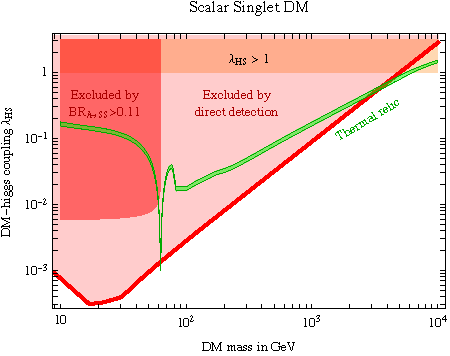
\includegraphics[width=0.6\textwidth]{figs/ScalarSinglet2023}
\caption[Scalar singlet DM]{\em  {\bfseries Scalar singlet DM}.
In the $(M,\lambda_{\rm HS})$ plane we plot the region excluded by direct detection,
the band favoured by the thermal DM abundance, and the region where
the quartic coupling is bigger than unity.
\label{fig:ScalarSinglet}}
\end{center}
\end{figure}


The most economical DM model, at least in terms of new degrees of freedom,
consists of adding a real neutral singlet scalar $S$ to the SM~\cite{ScalarSinglet}, and imposing an ad-hoc global symmetry $S\to -S$,
to make $S$ stable.
The most general renormalizable Lagrangian is then given by 
\beq 
\bbox{\Lag =\Lag_{\rm SM } + \frac{(\partial_\mu S)^2}{2} - \frac{m_S^2}{2} S^2 -\lambda_{HS} S^2 |H|^2- \frac{\lambda_S}{4} S^4}\ , 
\label{eq:LScalarSinglet}
\eeq
and contains, besides the kinetic and mass terms
for $S$, also a quartic scalar interaction between $S$ and the Higgs doublet $H$, and the phenomenologically mostly irrelevant quartic self-coupling, $S^4$.\footnote{Global symmetries might be broken by Planck mass suppressed operators, in which case DM could be made stable by considering a more complicated model, based on a local $\mathbb{Z}_2$ symmetry.
Such a $\mathbb{Z}_2$ symmetry could be, for instance, a remnant of a  dark $\U(1)$ gauge group, under which $S$ has a charge 1,
 spontaneously broken by the vacuum expectation value of another scalar, $S'$, with charge 2. This set-up would result in a distinct phenomenology: the complex $S$ would contain
two mass--split components, with the splitting induced by the $SSS^{\prime *}$ cubic interaction (see \arxivref{1407.6588}{Baek et al.~(2014)}~in~\cite{ScalarSinglet}).}
After the higgs field obtains its vev, $v \approx 174$ GeV, the DM mass is given by $M^2 = m_S^2 + 2\lambda_{HS} v^2$.
This must be positive, so that $\langle S\rangle = 0$, and $S$ remains stable.

The spin-independent direct detection DM scattering cross section is given by~\cite{ScalarSinglet}
\beq\label{eq:f} \sigma_{\rm SI}
= \frac{\lambda_{HS}^2 m_N^4 f_N^2}{\pi M^2 M_h^4}, 
\eeq
where $f_N\approx 0.3$
is the nucleon matrix element 
(see section~\ref{sec:benchmark:models}),
$M_h \approx 125$ GeV is the higgs boson mass,
$m_N=0.939$~GeV is the nucleon mass
and  for simplicity $m_N \ll M$ was assumed in order to shorten the expression.
The DM relic abundance is set by the thermal freeze-out (see section~\ref{sec:thermal_relic}), where
the non-relativistic $s$-wave $SS$ annihilation into SM particles can proceed in two ways: (i) via $SS\to h\to f \bar f$, where $f$ is any kinematically accessible SM final state, i.e., any SM fermion or gauge boson for which~$m_f < M$, and (ii) via direct $SS \to hh$ annihilation, possible if $M_h < M$.
The result is~\cite{ScalarSinglet}
\beq
\label{eq:sigmav:SingletDM}
\sigma v = \frac{16\lambda^2_{HS} v^2}{\big(4M^2 - M_h^2\big)^2 + M_h^2 \big( \Gamma_h(M_h)+\Gamma_{h\to SS}\big)^2} \frac{\Gamma_h(2M)}{2M}
+\frac{\lambda^2_{HS}}{64\pi M^2} \sqrt{1-\frac{M_h^2}{M^2}} \Theta(M-M_h),
\eeq
where the $h\to SS$ partial decay width, for $M_h>M$, is given by
\beq
\Gamma_{h\to SS} = \frac{\lambda^2_{HS} v^2}{4\pi M_h}\sqrt{1-4\frac{M^2}{M_h^2}}.
\eeq 
The second term in eq.~\eqref{eq:sigmav:SingletDM} accounts for the  $SS \to hh$ annihilation channel, with $\Theta$ the step function. The first term in \eqref{eq:sigmav:SingletDM} accounts for the $SS\to h\to f \bar f$ channel, and has the Breit-Wigner form due to the intermediate Higgs  resonance. It is expressed in terms of $\Gamma_h(m)$, the total decay width of a SM Higgs boson, had it had mass equal to $m$. The tabulated values for $\Gamma_h(m)$ can be found, e.g.,~in \cite{hdecaywidth}.
For $M\gg M_W$ the expression for the annihilation cross section eq.~\eqref{eq:sigmav:SingletDM}
 tends to its $\SU(2)_L$-invariant limit, thanks to the apparent non-decoupling of the $\Gamma_h(m)$ factor. 
Note that the $S^4$ quartic coupling helps in maintaining the kinetic equilibrium also close to the Higgs resonance, $M \approx M_h/2$, where the annihilation is resonantly enhanced,
such that this regions remains allowed by direct detection bounds.


In fig.\fig{ScalarSinglet} we show with dark red shading
the region in the $(M,\lambda_{\rm HS})$ plane  that is excluded by the bounds on the invisible width of the higgs, i.e., in the excluded region ${\rm BR}(h\to SS)>0.11$~\cite{htoinvisibles}. 
The region excluded by direct DM searches is shown with light red shading, 
and the band where the thermal relic DM density reproduces the measured DM density $\Omega_{\rm DM}$ by a green band.
Indirect detection bounds could also be added on the same plane but turn out not to be very relevant.

 In this simple model a single coupling, $\lambda_{HS}$, controls both the relic density abundance and the direct detection scattering cross section, since both involve either a Higgs exchange or Higgs production. It is therefore possible to fully test the model in different, complementary ways. Assuming there are no other production mechanism beside thermal DM production, the model is allowed only for DM that is heavy enough, $M \gtrsim 3\TeV$.
 There is also an upper bound on DM of about 7 TeV, since for larger DM masses the thermal annihilation cross section requires large couplings, $\lambda_{HS}\circa{>}1$,
 and thus runs afoul of perturbativity bounds. 
 Since only a finite DM mass interval remains viable, future experiments can in principle cover the whole parameter space of the model.

\bigskip

In the complex $S$ version of the model, DM can be stable after imposing either $\mathbb{Z}_2$, $\mathbb{Z}_3$, or U(1) global symmetries, 
or an invariance under complex conjugation  $S\to S^*$~\cite{scalarZ3DM}.
The latter symmetry remains unbroken even for $\langle S\rangle\neq0$,
such that $\Im S$ remains a stable DM candidate.
The Lagrangian for the $\mathbb{Z}_3$ model is given by
\beq 
\Lag =\Lag_{\rm SM } + |\partial_\mu S|^2 - m_S^2 |S|^2 -\lambda_{HS} |S|^2 |H|^2- \lambda_S |S|^4 + A (S^3 + S^{*3}) .\label{eq:LScalarSingletZ3}
\eeq
DM is stable despite the cubic $S^3$ interaction, as the action is invariant under a $S\to e^{2\pi /3} S$ realising a
$\mathbb{Z}_3$ symmetry.
If DM is the pseudo-Goldstone phase of a complex $S$
with spontaneously broken U(1) symmetry,
its interactions get suppressed at low energy, reducing direct detection bounds~\cite{1708.02253}.





\begin{figure}[t]
\begin{center}
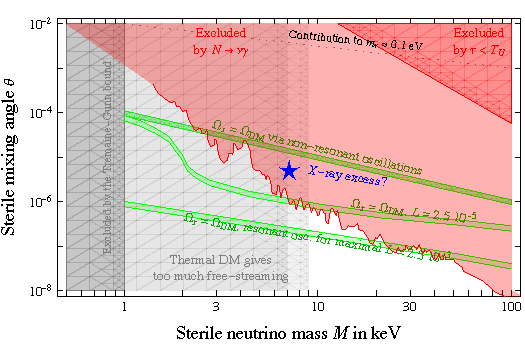
\includegraphics[width=0.68 \textwidth]{figs/SterileDM} 
\end{center}
\caption[Sterile neutrino]{\em \label{fig:SterileDM}  {\bfseries Sterile neutrino DM}. 
The red region is excluded from DM decays into $X$-rays~\cite{SterileNu}, 
while in the dark red region DM  also has a lifetime that is shorter than the age of the Universe. 
Production via non-resonant neutrino oscillations reproduces the DM abundance in the upper green band,
while resonant oscillations give the lower green bands, which assume the indicated lepton asymmetry~\cite{SterileNu}.
The light gray region below $M < 9\keV$ is excluded by free-streaming, if DM has thermal velocity;
such bound becomes somewhat weaker, if DM has a mildly sub-thermal velocity distribution (mid-dark gray).
Below the dotted line the $N$ contribution to the active neutrino masses is below their observed values.
The star indicates the possible $3.5\keV$ excess, discussed in section~\ref{sec:3.5keV}. 
}
\end{figure}






\subsection{Fermionic singlet DM: `sterile neutrino'}\label{FermionSinglet}\index{Sterile neutrino}\index{DM theory!sterile neutrino}

Another minimal choice for a DM model is to add to the SM an extra neutral Weyl fermion $N$. Here, one faces a choice of whether or not to impose the ad-hoc $N\to -N$ symmetry, similarly to what was done in section \ref{ScalarSinglet} for the scalar singlet DM. Imposing the $N\to -N$ symmetry makes $N$ stable, but also means that there are no renormalizable interactions between $N$ and the SM (in contrast to the scalar singlet DM, where one can still write down the Higgs quartic $S^2|H|^2$ term, see eq.~\eqref{eq:LScalarSinglet}), making the production of DM in the early universe an unresolved question. 
One could introduce both $N$ and an extra scalar singlet $S$ (or, alternatively, a vector singlet);
however the resulting models~\cite{FermionicSinglet} would lead us away from minimality.

\smallskip

Dropping the requirement of an $N\to -N$ symmetry is a much more widely discussed possibility, that goes under the name of a {\em sterile neutrino} or {\em right-handed neutrino}, and we thus focus on it. The attractive feature is that one can 
now write down a Yukawa interaction between $N$, the left-handed leptons $L$ of the SM, and the Higgs doublet $H$:
\beq
\label{eq:sterile:Lag}
\bbox{\Lag=\Lag_{\rm SM} + \bar N i \slashed{\partial} N + 
\left(M \frac{N^2}{2} + y\,NLH  + \hbox{h.c.}\right)}~.
\eeq
 In fact, adding two or three
right-handed neutrinos $N_i$, with a Majorana mass matrix $M$ and Yukawa couplings $y_{ij}\,N_i L_j H $
is the simplest extension of the SM that at low energies reproduces the small sizes of neutrino masses via the see-saw mechanism, $m_\nu = v^2\, y^T M^{-1} y$, after the heavy degrees freedom $N_i$ are integrated out. 
In this context, one often considers heavy sterile neutrinos with masses $M \sim 10^{10}\GeV$ such that $y \sim 1$. This set-up also leads to a successful 
baryogenesis via leptogenesis already in  its minimal implementation (see~\cite{BaryoLeptogenesis} for reviews).

For DM the more interesting region of the parameter space is if the sterile neutrino has a mass $M \circa{>}\keV$~\cite{SterileNu},
just above the Gunn-Tremaine bound for fermionic DM, see eq.\eq{GunnTremaine}. 
This then leads to a viable DM candidate, albeit a decaying one.
For such light $N$ the Yukawa coupling $y$ needed for the see-saw
becomes small enough so that the sterile neutrino is stable on cosmological time-scales. Working to first nonzero order in small $y$, 
the interactions of $N$ with the light SM fields are the same as for the active SM neutrinos, but suppressed by the mixing angle between the sterile neutrino and the active neutrinos, $\theta = y v/M \ll1$.\footnote{We use a single angle $\theta$ that describes mixing of $N$ with a particular linear combination of $\nu_e, \nu_\mu, \nu_\tau$, since for our discussion the SM neutrino flavors are irrelevant. For production of $N$, for instance in $\nu_e$ or $\nu_\mu$ scattering on target, on the other hand, one needs to distinguish between different mixing angles for each SM neutrino flavor.}
For $M < m_e$  the dominant decay mode of $N$ is into active neutrinos, with the decay width given by~\cite{nustau}
\beq\Gamma(N\to 3 \nu) =\frac{G_{\rm F}^2 M^5}{96\pi^3}\theta^2 \approx \frac{\theta^2}{33 \, T_{\rm U}} \left(\frac{M}{\keV}\right)^5.\eeq
This partial decay width (that dominates the DM lifetime $\tau$)
must be longer than the age of the universe,
$ \tau \approx 1/\Gamma(N\to 3\nu) \gtrsim T_{\rm U}=13.7~{\rm Gyr}$.
As shown in fig.\fig{SterileDM}, this bound would allow for sterile neutrino DM that gives the right contribution to neutrino masses (which occurs along the dotted black line in the upper part of the figure).
However, significantly stronger bounds on sterile neutrino decays follow from the modes that include photons,
since photons are much easier to detect.
The dominant such decay mode is $N\to \nu\gamma$, arising at one-loop level. 
The corresponding partial decay width is
\beq\label{eq:N->nugamma}
\Gamma(N \to \nu \gamma)=\frac{9 \alpha G_{\rm F}^2M^5}{256\pi^4 }\theta^2 
 \approx \frac{\theta^2}{4250 \, T_{\rm U}}  \bigg(\frac{M}{\keV}\bigg)^5.\eeq
Observations require  $\tau \, \hbox{BR}(N \to \nu \gamma)=1/\Gamma(N \to \nu \gamma)\gtrsim 10^8 \,T_{\rm U}$,
with the precise bound shown in fig.~\ref{fig:SterileDM} as a light red shaded region.
This implies that the $N$ contribution to neutrino masses, $m_\nu = M \theta^2 $, 
is smaller than about $0.04\ \text{eV}\big(\text{keV}/M\big)^4$, and thus smaller than the largest difference between SM neutrino masses. This means that there needs to be additional contributions to SM neutrino masses beyond the see-saw type contribution due to mixings with the sterile neutrino DM. 


\subsubsection{Freeze-in via non-resonant oscillations} \index{DM cosmological abundance!freeze-in}\index{Sterile neutrino!Dodelson-Widrow mechanism}\index{Dodelson-Widrow mechanism}
The same mixing angle $\theta$ also controls the production of sterile neutrino DM in the early Universe. 
In the dense plasma, active-sterile oscillations are averaged by the decoherent scatterings on matter, and the production process can be seen as a version of the freeze-in mechanism (section \ref{Freeze-in}).
At a temperature $T\ll M_Z$ the interaction rate of the sterile neutrino with the thermal bath 
is given by $\Gamma_{\rm s} \approx \theta_m^2  \Gamma_\nu$, where $\Gamma_\nu$ is the interaction rate of any of the three active neutrinos~\cite{SterileNu}.
 The modified active/sterile mixing angle\footnote{The full expressions provided in the literature \cite{SterileNu} reduce to this compact approximated formula for $\theta \ll 1$.}, 
$\theta_m  \approx \sfrac{\theta}{(1+{\mathcal O}(1)T^6 G_{\rm F}^2/\alpha M^2)}$, includes the effects due to finite density and finite temperature. 
The ratio between $\Gamma_s$ and the Hubble rate,
\beq
 \frac{\Gamma_{\rm s}}{H} \approx  \theta_m^2 \left(\frac{T}{3\,{\rm MeV}}\right)^3,
 \eeq
is maximal at  $T_* \approx  130\,{\rm MeV} (M/{\rm keV})^{1/3}$
and results in the following amount of sterile neutrinos, as measured in terms of new fermionic, relativistic degrees of freedom $\Delta N_\nu$ (contributions to $\Delta N_{\rm eff}$, see eq. \eqref{eq:DeltaNeff} in App.~\ref{sec:app:particles:thermal}):
\beq \label{eq:sterileOscAb}
\Delta N_\nu \approx \min\left (1, \max_T \frac{\Gamma_{\rm s}}{H}\right)\approx \min\left(1,10^6\, \theta^2 \frac{M}{\keV}\right).
\eeq
The mass abundance at low temperatures, when sterile neutrinos are well in the non-relativistic regime,  is then $ \Omega_{\rm s} h^2 = \Delta N_\nu \cdot \sfrac{M}{94\eV} $, see eq.~\eqref{eq:rhonu}.
This production mechanism is also referred to as the {\bf Dodelson-Widrow mechanism}. It leads to sterile neutrinos with a roughly thermal velocity.



The upper green band in fig.\fig{SterileDM} shows the region of parameter space in which sterile neutrino production via non-resonant oscillation reproduces the observed cosmological DM abundance. However, a combination of the bound from $X$-rays due to DM decays
(red region) and on DM free-streaming (eq.\eq{WarmDMbounds}, gray region) excludes the possibility of a DM production via non-resonant oscillations. The following assumptions went into the prediction for DM abundance: {\em i)} that there were basically no sterile neutrinos in thermal plasma at temperatures above about 1 GeV, {\em ii)} that the only sterile neutrino interactions are the ones induced from mixing with the active SM neutrinos; 
{\em iii)} that the Universe has no lepton asymmetry at temperatures below 1 GeV. 
Violating one or more of the above assumptions can change the predictions, where a notable example is the freeze-in via resonant oscillations, discussed below. 



\subsubsection{Freeze-in via resonant oscillations} \index{Sterile neutrino!Shi-Fuller mechanism}\index{Shi-Fuller mechanism}
Since the sterile neutrino is heavier than the active neutrinos, 
resonant oscillations can only happen due to in medium effects. 
If the thermal plasma has a lepton asymmetry, this creates an effective mass term for neutrinos.\footnote{More precisely, thermal effects induce a term in a dispersion relation that is linear in the neutrino energy, and to which the forward scatterings of neutrinos on neutrinos in a thermal plasma give opposite contributions then do the scatterings 
of neutrinos on antineutrinos. This effect therefore vanishes for $n_\nu =n_{\bar \nu}$ \cite{Noztold:Raffelt}.}
 The changed dispersion relation for active neutrinos can be similar to the dispersion for sterile neutrinos, for some particular momenta. This level crossing transfers the leptonic excess from active neutrinos into the sterile neutrinos. The resulting sterile neutrino DM relic abundance is roughly proportional to the lepton asymmetry, $L=(n_\nu-n_{\bar \nu})/(n_\nu+n_{\bar \nu})$ (we assume that there is no lepton asymmetry in the charged leptons sector, in agreement with observations). This mechanisms is also known as the {\bf Shi-Fuller mechanism}. For it to work, $L$ needs to be much larger than the baryon asymmetry, by at least 5 orders of magnitude. 

Furthermore, the minimal model with 3 sterile neutrinos can also produce baryogenesis together with the large lepton asymmetry $L$,
provided that the CP-asymmetry is enhanced by having 2 quasi-degenerate heavier sterile neutrinos.
The scatterings that produce the two heavy sterile neutrinos first result in a lepton asymmetry, which then
gets converted into a baryon asymmetry via sphalerons. This process is active only at temperatures above the electroweak scale, i.e., before the sphalerons decouple~\cite{SterileNu}.
The scatterings at lower temperatures still continue to produce a lepton asymmetry, which thereby is bigger than the baryon asymmetry  ---
possibly  almost as big as the maximal
lepton asymmetry allowed by the BBN constraints, $L \circa{<} 2.5~10^{-3}$~\cite{SterileNu}. This lepton asymmetry then gets converted into relic abundance of the lightest sterile neutrino state, $N_1$, via resonant oscillations.

If the  sterile neutrino DM state $N_1$ is produced through resonant oscillations, it tends to have a sub-thermal average velocity, since the  level crossing happens predominantly for lower $N_1$ momenta. The sterile neutrino DM is then less warm than if it were produced via a thermal freeze-out, 
and thereby the bounds from free-streaming are weaker, roughly $M \circa{>} 7\keV$ (\arxivref{1706.03118}{Baur et al.~(2017)} in~\cite{SterileNu}).


\subsubsection{Freeze-in via decays}
The complications, such as the need for a large lepton asymmetry $L$, which are encountered in the minimal scenario, 
motivate the  investigations of other, non-minimal, production mechanisms that could result in a production of
relatively cold sterile neutrinos~\cite{SterileNu}.
The simplest possibility would be a freeze-in production from the Higgs decays. 
However, in this case eq.\eq{decayfreezein} implies a too large value of the Yukawa coupling $y$ in eq.~\eqref{eq:sterile:Lag},
and thereby a too fast $N\to\nu\gamma$ decay according to eq.\eq{N->nugamma}.
One needs to introduce extra particles, such as a
scalar singlet $\phi$ with a Yukawa interaction $\phi N^2$ 
or a vector lepto-quark ${\cal U}$ with a gauge-like interaction 
$( \bar u_R^i \gamma^\mu N) {\cal U}_\mu$, which then set the relic abundance.
Note that, similarly to the freeze-in via resonant oscillations, the freeze-in production of $N$ via decays, with a partially closed phase space, also
gives rise to the sterile neutrino DM with a sub-thermal velocity distribution. The bound on the mass of warm DM
quoted in eq.\eq{WarmDMbounds} can therefore be appreciably relaxed, so that the sterile neutrinos could even have a mass $M = 7\keV$. This is, for instance,
needed to fit the possibly anomalous 3.5 keV $X$-ray line discussed in section~\ref{sec:3.5keV}.


The viable parameter space of models can be further enlarged, if one can invoke some mechanism that dilutes the abundance of sterile neutrinos after the freeze-in era completes, such as an entropy release into other particles at some later time~\cite{SterileNu,DM:entropy:injection}.


\subsection{Vector singlet DM}\label{VectorSinglet}
\index{Vector singlet}\index{DM theory!vector singlet}
Building on the theme of DM models with minimal number of extra degrees of freedom discussed
in the previous sections, one can also consider adding to the SM a vector singlet $A$~\cite{VectorSinglet}. 
A $A^\mu \to -A^\mu$ symmetry (either imposed by hand or inherited by other reasons, see section \ref{sec:DMSSB} and \cite{VectorSinglet}) can guarantee the stability of $A$.
Then, a possible effective Lagrangian is  
\beq 
\Lag =\Lag_{\rm SM } -\frac14 F^{\mu\nu}F_{\mu\nu} + \frac{M_A^2}{2} A_\mu A^\mu +\frac{\lambda_{HV}}{2} A_\mu A^\mu |H|^2 - \frac{\lambda_V}{4} (A_\mu A^\mu)^2\ , 
\label{eq:LVectorSinglet}
\eeq
up to issues related to gauge invariance.
The mass term $M_A$ can be generated by a St\"uckelberg or Higgs mechanism in the hidden sector.
Extra scalars are needed in the latter case.


This model features a phenomenology similar to the scalar singlet DM discussed in section~\ref{ScalarSinglet}~\cite{VectorSinglet}. 
The typically considered mass range is around the weak scale. In the sub-GeV mass range, the model corresponds to the dark photon, see section \ref{sec:VectorPortal}. 




\section{Dark Matter charged under the SM group}

\subsection{Charged Dark Matter}\label{sec:ChargedDM}
Observational constraints essentially exclude DM with an electric charge comparable to the electron charge $e$.
DM could, however, carry a fraction of a unit charge. This possibility goes under the name of milli-charge DM, and was reviewed in section \ref{sec:milicharged}.

\subsection{Colored Dark Matter}\label{sec:ColoredDM}\index{DM properties!strong interactions}
Moving to color,
could additional particles $Q$ charged under QCD constitute the DM? Any such colored particles would be confined inside hadrons, i.e., bound states that are singlets under $\SU(3)_c$. 
Given that hadrons continue to have strong interactions, there are stringent bounds on such scenarios, even in the least constrained case where additional colored particles only form neutral hadrons  so that the bounds on charged DM are avoided.
The hadrons containing valence light quarks $q=\{u,d\}$ (such as $QQ q$ and $Q qq$) and/or gluons are $\approx 1/\Lambda_{\rm QCD}$ in size. The cross section for scattering of such DM on nucleons is therefore $\sigma_{\rm SI} \approx \pi/\Lambda_{\rm QCD}^2 \approx 1.6~10^{-26}\cm^2$. 
Such DM candidates have been excluded up to masses $M \sim 10^{15}\GeV$ or slightly higher, as discussed in section~\ref{sec:SIMP}.


The remaining allowed DM candidates are 
neutral hadrons that have as constituents {\em only} the new stable colored particles $Q$, 
with masses $M_Q\gg \Lambda_{\rm QCD}$.
The hadrons are then made out of, e.g., $QQ$ if $Q$ is a color octet, and out of $QQQ$ if $Q$ is a triplet, with both options resulting in
viable DM candidates~\cite{coloredDM}. 
The hadrons are  bound states of a Coulomb-like potential,
with large binding energies, $E_B \approx \alpha_{\rm s}^2 M_Q$, and of small sizes on the order of $1/\alpha_{\rm s} M_Q$,
such that the bound states have small residual QCD interactions.
The study of their phenomenology (see e.g.~\arxivref{1801.01135}{De Luca et al.~(2018)} \cite{coloredDM}) shows that they are viable DM candidates for multi-TeV masses:
the  direct detection cross section $\sigma \sim \Lambda_{\rm QCD}^4/M_Q^6$ satisfies
the present bounds for $M_Q\circa{>}10\TeV$;
the cosmological DM abundance is reproduced thermally for $M_Q \approx 12.5\TeV$ for a color octet;
the indirect detection rates, dominated by recombination, e.g.,\ $QQ+\bar Q\bar Q \to Q\bar Q+Q\bar Q$, are below the present bounds, while
the collider bounds are satisfied for $M_Q\circa{>}(1-2)\TeV$.


This kind of DM is allowed if, during the cosmological evolution, essentially only the bound states made of $Q$ are formed and the production of problematic bound states that contain ordinary light quarks is sufficiently suppressed.
In the limit where all the interactions are much faster  than the Hubble rate,
the cosmological evolution leads to the production of states made out of only $Q$, because these have a bigger binding energy
$E_B \gg \Lambda_{\rm QCD}$.
Estimates of the relevant QCD rates suggest that the problematic
hadrons have an abundance that is a few orders of magnitude smaller than
the $Q$-only hadrons.
Such a small abundance is allowed by the bounds on the strongly-interacting
relics, as discussed in section~\ref{sec:SIMP}.
Furthermore, such states lead to an unusual DM signal: 
heavy hadrons that hit the upper atmosphere and then slowly sink, remaining
in normal matter as rare heavy atoms, and could potentially be discovered in this way.
Searches with excited tantalum, in particular, could probe them, since they can be sensitive to very small DM abundances (see \arxivref{1911.07865}{Lehnert et al.~(2020)} in~\cite{SIMP}).


\subsection{Weakly Interacting Massive Particles}\label{sec:WIMPs}\index{WIMP}\index{DM properties!weak interactions}\index{DM!as weak-scale particles}
Weakly Interacting Massive Particles (WIMPs) are a class of particles that play a prominent role as DM candidates. 
Perhaps because of their prominence, the definition of a WIMP is not entirely clear-cut.



In the narrowest sense, WIMP refers to a particle that interacts with the $W$ and $Z$ electroweak bosons.
Therefore, a DM candidate classified as a WIMP needs to be charged under the electro-weak part of the Standard Model gauge group, $\SU(2)_L\otimes \U(1)_Y$, 
have zero electromagnetic charge, be a color singlet, and be stable.
If the WIMP has a weak-scale mass, $M \sim M_{W,Z}\sim 100\GeV$
(usually interpreted loosely, up to several orders of magnitude), then 
the annihilation cross section of two WIMPs is comparable to what is required 
for the simplest thermal freeze-out mechanism to generate the observed cosmological DM abundance, 
see the discussion surrounding eq.\eq{rhoDMestimate} in  section~\ref{sec:thermalapprox}.
In scenarios with multiple WIMPs, the lightest WIMP can be the Dark Matter, while
co-annihilations may play an important role, see section~\ref{sec:coann}.

\smallskip

When interpreted more broadly, however, 
the term WIMP is used to denote a stable particle, 
which couples to other weak-scale particles such as the Higgs or the top quark in the SM,
has interactions {\em `as weak as'} the $\SU(2)_L\otimes \U(1)_Y$ gauge interactions of the Standard Model, 
and therefore also has a {\em `weak-scale-like'} annihilation cross section. Clearly, a much wider set of models falls under the WIMP moniker in this case, thus making the WIMP assumption less predictive. 
Although there is no longer a direct connection to the SM weak interactions, the WIMP mass is still typically taken to be around 100 GeV.
For adequately chosen parameters the correct relic abundance is still set by thermal freeze-out, in which case the phenomenology of broadly defined WIMPs is 
similar to the WIMPs defined more literally. 

\medskip

Historically, the simplicity of the freeze-out production mechanism, and the fact that DM could be connected to the stabilization of the electroweak scale against quantum corrections (the solutions to the hierarchy problem, as discussed in the next chapter), made WIMPs stand out as a conceptually attractive DM candidate since the early 1980's. This focus on WIMPs was aligned with the focus on low energy supersymmetry, which during that period was the motivation for most of the beyond the SM searches. In fact, for many years WIMP and neutralino, the lightest neutral supersymmetric particle (see section~\ref{sec:SUSYDM}), were colloquially essentially synonymous. 
The motivation was strong enough that it jump-started a large experimental program aimed at discovering WIMPs in either direct detection, indirect detection, or production at colliders. 

So far, this large experimental program only resulted in bounds. 
While the WIMP idea is by no means excluded, the absence of a discovery did result  in a shift and broadening of the experimental and theoretical focus  in the last decade, which we extensively covered in the present review. 

\medskip

A specific realization of WIMPs, intended in the stricter sense given above, is the Minimal Dark Matter hypothesis, which is discussed in the following subsection. Many of the other WIMP candidates, that belong to either the stricter or the broader categories, such as neutralinos or extra-dimensional DM, are discussed in chapter \ref{BigDMtheories}.





\begin{table}[t]
\begin{center}
\small
$$\begin{array}{|cccc|c|cc|cc|}\hline
\multicolumn{4}{|c|}{\hbox{Quantum numbers}}
&\hbox{DM could}& \multicolumn{2}{c|}{\hbox{$M_{\rm DM}$ in TeV}}&M_{{\rm DM}^\pm} \!-\! M_{\rm DM}\!\!\!&
 \hbox{$\sigma_{\rm SI}$ in}  \\
\!{\rm U}(1)_Y\! \!& \! \!\SU(2)_L\! \!&\!\!\SU(3)_c\! \!& \hbox{Spin} &
 \hbox{decay into} & \hbox{tree}  & \hbox{non-pert} &\hbox{in MeV} &
 \hbox{$10^{-46}\,{\rm cm}^2$} \\ \hline
 \hline \rowcolor[rgb]{0.9,0.95,0.95}
1/2 &2 & 1 & 0 & EL & \multicolumn{2}{c|}{0.54}  & 350 & (0.4\pm 0.6)\,10^{-3} \\  \rowcolor[rgb]{0.9,0.95,0.95}
1/2  & 2&1& 1/2 & EH & \multicolumn{2}{c|}{1.1}  & 341 & (0.3\pm 0.6)\,10^{-3}\\   \rowcolor[rgb]{0.95,0.95,0.85}
\hline
0&3&1&  0 & HH^* & 2.0&  2.5  & 166& 0.23\pm 0.04 \\  \rowcolor[rgb]{0.95,0.95,0.85}
0&3&1 & 1/2 & LH & 2.4&  2.6  & 166 & 0.23\pm 0.04\\  \rowcolor[rgb]{0.95,0.95,0.85}
1&3&1& 0 & HH,LL & 1.6&  \,?  & 540 &0.001\pm 0.001\\ \rowcolor[rgb]{0.95,0.95,0.85}
1&3 & 1 & 1/2 & LH & 1.9& \, ? & 526  & 0.001\pm 0.001\\ \rowcolor[rgb]{0.95,0.95,0.95}
\hline
1/2  & 4 &1 & 0 & HHH^* & 2.4& \,?  & 353 & 0.27\pm 0.08\\  \rowcolor[rgb]{0.95,0.95,0.95}
1/2 &4 & 1& 1/2 & (LHH^*) & 2.4& \,?  & 347  & 0.27\pm 0.08\\  \rowcolor[rgb]{0.95,0.95,0.95}
3/2 &4 & 1& 0 & HHH & 2.9& \,? & 729 & 0.15\pm 0.07\\  \rowcolor[rgb]{0.95,0.95,0.95}
3/2  &4 & 1& 1/2 & (LHH) & 2.6& \, ?  & 712  &0.15\pm 0.07\\  \rowcolor[rgb]{0.85,0.95,0.85}
\hline
0 & 5 &1 & 0 & (HHH^*H^*) &5.0 &  14  & 166  & 2.0\pm0.5\\   \rowcolor[rgb]{0.85,0.95,0.85}
0 & 5 & 1 & 1/2 & \hbox{none} &4.4 &  14  & 166 & 2.0\pm0.5 \\  
\hline
\end{array}
$$
\color{black}
\normalsize
\caption[Minimal Dark Matter properties]{\em {\bfseries Minimal Dark Matter}. The first columns define the quantum numbers of the possible DM weak multiplets.
The following ones show: the possible decay channels into SM particles that need to be forbidden (those in parenthesis correspond to dimension-5 operators);
the DM mass predicted from thermal abundance (either at tree level, left column, or including non-perturbative
Sommerfeld and bound-state corrections, right column, the latter not computed in all cases);
the predicted splitting between the charged and the neutral components of the DM weak multiplet;
the prediction for the SI DD cross section $\sigma_{\rm SI}$. 
\label{tab:MDM}}
\end{center}
\end{table}



\subsection{Minimal Dark Matter}
\label{MDM}
\index{Minimal DM}\index{DM theory!Minimal}\index{DM properties!weak interactions}
A DM model of the Minimal Dark Matter (MDM) type is a minimal extension of the SM 
where a single DM multiplet is added
to the SM~\cite{MDM}. 
Many non-minimal models reduce to MDM in the limit  where only one added field is relevant for DM. 
For instance, a supersymmetric wino (section \ref{Wino}) corresponds to an added triplet in the MDM context when it is `pure', i.e.~unmixed with other supersymmetric fermions. 
We will shortly mention several of such cases, and for that let us first consider the MDM set-up systematically.

\medskip

The non-trivial multiplets charged under the 
SM gauge group $\mathcal{G}_{\rm SM} = {\rm U}(1)_Y\otimes\SU(2)_L\otimes\SU(3)_c$ 
that can be added to the SM and that contain elementary particles that can be
acceptable DM candidates are listed in table~\ref{tab:MDM}.
In order to be acceptable, DM must have a vanishing color and electric charge\footnote{More precisely, the charge needs to be negligibly small from observation, see section~\ref{sec:milicharged}: 
in the case of discrete choices, this leaves $Q=0$ as the only option.
Special colored multiplets can give allowed DM as QCD bound states, as discussed in section~\ref{sec:ColoredDM}.
The case of singlets of the SM gauge group has been considered in 
section~\ref{ScalarSinglet} (scalar singlet) and~\ref{FermionSinglet} (fermion singlet), so they are not reported here.} 
\beq
Q=T_3+Y=0,
\eeq 
where $Y$ is the hypercharge of the electroweak multiplet and $T_3$ the corresponding eigenvalue of the diagonal generator of $\SU(2)_L$.
The most prominent examples are discussed in detail:
\begin{itemize}
\item[$2_S$] The first possibility is the  {\bf inert Higgs doublet} model, also called the {\bf Inert Doublet Model (IDM)}, where the SM field content is supplemented by the complex $H' = (h^{\prime +}, h^{\prime 0})$ field: 
a scalar weak doublet with $Y=1/2$,
which contains a complex neutral component $h^{\prime 0}$ in its lower component, with $T_3 = -1/2$,
and a charged component in its upper component, with $T_3=-1/2$.
An ad-hoc symmetry such as $H'\to - H'$ is needed to make  it stable.
The inert Higgs doublet $H'$ has the same gauge quantum numbers as the SM Higgs,  $H$. In supersymmetry, this field would be called the {\em left-handed slepton} $\tilde{L}$. The phenomenology of inert Higgs doublet model
is discussed in section~\ref{sec:inertHiggs}.

 
 \item[$2_F$] The second possibility is a {\bf higgsino-like} fermionic weak doublet with $Y=1/2$. In supersymmetric models this field arises
 as a fermionic partner of the Higgs scalar.  An ad-hoc symmetry is again needed in order to forbid the otherwise allowed
 renormalizable couplings to the SM fields, which, if present, would make the higgsino unstable.
 
 \item[$3_F$]
 Yet another possibility is a fermionic weak triplet, which can have $Y=0, 1$. The $Y=0$ case corresponds to the mentioned {\bf wino-like} DM~\cite{Wino}, the fermionic partner of the $\SU(2)_L$ vectors in supersymmetric models (section \ref{Wino}). In these models the wino-like DM limit arises when 
  all  supersymmetric interactions are irrelevant, and therefore all the interactions are dictated by
 the gauge quantum numbers.
Also in this case, additional ad hoc symmetries,  such as a $\mathbb{Z}_2$ or U(1)$_{B-L}$, 
 are needed in order to forbid extra renormalizable couplings that would otherwise make the wino-like state unstable.
 
 
\item[$3_S$]  {\bf Scalar triplets} with $Y=0$ or 1 provide additional DM candidates, 
that, however, also need to be stabilised by invoking ad-hoc symmetries~\cite{MDM}. (The phenomenology of the $Y=0$ candidate
was also discussed in \cite{Arakawa:2021vih}.)

\item[$4$]  Various {\bf fermionic or scalar 4-plets} provide DM candidates, which yet again need ad-hoc stabilising symmetries.
Even though the fermionic 4-plets can only decay via dimension-5 operators, this by itself does not suppress enough the decay rates, and additional symmetries need to be invoked even in this case.
 
\item[$5_F$] The smallest multiplet that is automatically stable  is a {\bf fermionic quintuplet} (with one of the three possible $Y$ values,  $Y = 0,1,2$).
In this case all the interactions that can make the multiplet decay are 
 forbidden by gauge and Lorentz symmetries, up to dimension-6 operators. The dimension 6 operators result in a slow enough decay rate, 
 $1/\tau \sim M^5/\Lambda^4$,  if the suppression scale is  high, $\Lambda \sim M_{\rm Pl}$. 
 \end{itemize}
The list of phenomenologically interesting minimal DM candidates is finite, since the electroweak multiplets cannot be too larger 
in order not to result in a too fast renormalisation group running of the SU(2)$_L$ gauge coupling.  Requiring perturbativity up to $M_{\rm Pl}$ means that the fermions can be at most in a quintuplet, while (real) scalars can be at most in a 6-plet. Table~\ref{tab:MDM} therefore provides a relatively complete list of minimal DM candidates. Note that the 
6-plets, not listed in table~\ref{tab:MDM}, are not automatically stable, and their phenomenology is similar to the 4-plets. 

\medskip

Since the fermionic 5-plet is automatically stable, without requiring extra symmetries, 
and with no extra parameters apart from the DM mass, it is often referred to as {\em the Minimal DM} candidate.
 However, as mentioned at the beginning of the section, the notion of MDM is wider, and in general refers to
 a group of DM candidates with a similar phenomenology, 
 rather than to a single DM  candidate.
Importantly, in its most constrained version the MDM mass is fixed from the observed thermal abundance (see below), 
which means that the MDM model is fully predictive, without free parameters.

\bigskip

We now move to the phenomenology of MDM candidates. 
The full renormalizable Lagrangian of the model is given by (here ${\cal X}$ denotes the added multiplet):
\beq \label{eq:MDMlagrangian}
\bbox{\Lag = \Lag_{\rm SM} +c
\left\{\begin{array}{ll}
 \bar{{\cal X}} (i D\hspace{-1.4ex}/\hspace{0.5ex}+M) {\cal X} & \hbox{: ${\cal X}$ is a spin 1/2 fermionic multiplet,}\\
|D_\mu {\cal X}|^2 - M^2 |{\cal X}|^2& \hbox{: ${\cal X}$ is a spin 0 bosonic multiplet,}
\end{array}\right.}\eeq
where $c=1/2$ for a real scalar or a Majorana fermion
and $c=1$ for a complex scalar or a Dirac fermion. 
DM phenomenology is controlled by the gauge interactions of the ${\cal X}$ multiplet. These arise from the covariant derivative $D$, and are fully determined by the gauge quantum numbers. If ${\cal X}$ is a fermionic multiplet, then the multiplet mass $M$ is the only free parameter, which, furthermore, is determined by the relic abundance (see below), and thus all DM physics is fully predicted. If ${\cal X}$ is a scalar multiplet, extra quartic couplings are allowed,\footnote{Explicitly, they consist of $\Lag_{\rm non~minimal} \supset -c\, \lambda_H ({\cal X}^*  T^a_{\cal X} {\cal X})\, (H^* T^a_H H)- c\, \lambda'_H |{\cal X}|^2 |H|^2 - \lambda_{\cal X}  ({\cal X}^*  T^a_{\cal X} {\cal X})^2/2 -  \lambda'_{\cal X} |{\cal X}|^4/2$. Specific representations allow for extra quartic terms, 
such as the one relevant for the inert doublet model discussed in section~\ref{sec:inertHiggs}.} and therefore  the scalar case is `less minimal' (unless the quartic couplings are assumed to be negligible). 
This can be contrasted, for instance, with supersymmetry, which predicts many multiplets and the corresponding interactions among them.
However, as mentioned above, in the limit where the lightest supersymmetric particle is much lighter than the other states, its phenomenology reduces to the one of MDM. Such a limit is sometimes referred to as a `hot-spot', a predictive point in the otherwise large parameter space. In this sense, MDM candidates are hot-spots of more variegated theories. 

\medskip


\subsubsection{Mass splitting}

At tree-level, all the components of the multiplet ${\cal X}$ have the same mass $M$.
Since $\SU(2)_L$ is broken, however, quantum corrections split the components with electric charges $Q$ and $Q'$, so that at one loop we have
\beq   \label{eq:dMQ}
M_Q -  M_{Q'} =\frac{\alpha_2 M}{4\pi}\left\{(Q^2-Q^{\prime 2})s_{\rm W}^2 f\bigg(\frac{M_Z}{M}\bigg)+(Q-Q')(Q+Q'-2Y)
\bigg[f\bigg(\frac{M_W}{M}\bigg)-f\bigg(\frac{M_Z}{M}\bigg)\bigg]\right\}.
\eeq
The loop function equals $f(r)\stackrel{r\to 0}{\simeq}  2\pi r$ in the limit $M \gg M_{W,Z}$~\cite{MDM}.
In this limit the mass splitting can be understood as  simply  the Coulomb energy stored in the electric fields
that surround each component of the multiplet.
Such energy gives an additional contribution to the mass of a point particle.
For a point-like particle of any spin, which couples with coupling $g$ to a light abelian vector of mass $M_V$,
one therefore has
\beq  \delta M = \int d^3r \left[\frac{1}{2}(\vec\nabla \varphi)^2 + \frac{M_V}{2}\varphi^2\right]=
\frac{\alpha}{2} M_V + \infty,\quad\text{where}\quad
\varphi(r) = \frac{g }{4\pi r}e^{-M_V r}.\eeq
Summing the contributions of the $\gamma,Z,W$ gauge bosons gives eq.\eq{dMQ}.
Numerically, the mass splitting between DM and the next lightest state is $M_{Q=1}-M_{Q=0} = 166 \MeV$, for $Y=0$.

\medskip

\subsubsection{Direct detection of Minimal DM}\label{sec:MDMDD}\index{Direct detection!of Minimal DM}

\begin{figure}[t]
\centering
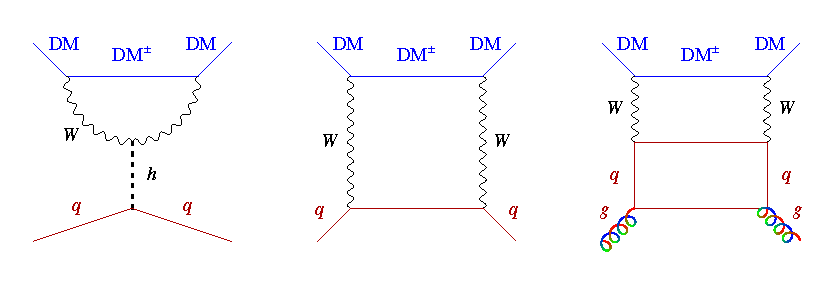
\includegraphics[width=0.9\textwidth]{figs/MDMsigmaSI} 
\caption[Minimal Dark Matter direct detection diagrams]{\label{fig:FeynLoopMDM}\em The main 1-loop and 2-loops Feynman diagrams relevant for direct detection of fermionic Minimal Dark Matter with $Y=0$.
}
\end{figure}

All MDM candidates with $Y\neq 0$ are excluded
because they have a vector-like interaction with the $Z$ boson 
with an order one coupling,  $-g_2 Y/\cos\theta_{\rm W}$.
At tree level, this produces a too large spin-independent elastic cross section on nuclei, 
see section~\ref{sec:SI},
\beq 
\label{eq:direct}
\sigma_{\rm SI}^A =c\frac{G_{\rm F}^2 m_A^2}{2\pi} Y^2(N - (1-4s_{\rm W}^2) Z)^2, 
\eeq
where $c=1$ for fermionic DM and $c=4$ for scalar DM, while $N$ and $Z$ are the neutron and proton content of the nucleus, respectively.
This cross section is a few orders of magnitude above the bounds from direct detection searches for $M \sim \TeV$,
see section~\ref{chapter:direct}.

The MDM candidates with $Y\neq 0$ 
are still allowed in non-minimal set-ups where the complex component of ${\cal X}$ with $Q=0$
is slightly mass split. The two resulting  real components cannot have vector interactions, thus avoiding direct detection bounds.
For an inert Higgs $H'$ this can be achieved  trough a renormalizable $(H' H^*)^2$ quartic coupling
(section~\ref{sec:inertHiggs}).
For a fermionic Higgsino this can be achieved by adding an extra real massive fermionic multiplet so that 
one can write down a Yukawa coupling with the SM Higgs; the extra fermion is either an electroweak singlet or a triplet (the latter possibility is automatically present in supersymmetric models).

\smallskip

Direct detection of MDM candidates with $Y=0$ (and of the MDM candidates with $Y\neq 0$ in the non-minimal set-ups)
proceeds via loop diagrams shown in fig.\fig{FeynLoopMDM}.
The scattering cross sections are the same for the case of either boson or fermion MDM, and are
suppressed by $1/M_W$ and $1/M_h$, rather than by $1/M$. The reason is that the 
scattering is dominated by the cloud of electro-weak vectors that surrounds the heavy DM particle.
In some cases, the accidental cancellations between the Higgs and the $W$-mediated one loop diagrams 
requires the computation of two-loop diagrams with external gluons.
The final results for the spin-independent cross sections are listed in table~\ref{tab:MDM} and plotted in fig.\fig{MDMOmega} (left): they are below the present bounds and above the neutrino fog. A future 50\,ton scale Xenon detector can thus exclude or discover all of the real MDM candidates ($Y=0$) and severly constrain the parameter space of complex MDM candidates with nonzero hypercharge (see \arxivref{2410.02723}{Bloch et al (2024)} in \cite{MDM}).

\begin{figure}[!t]
\begin{center}
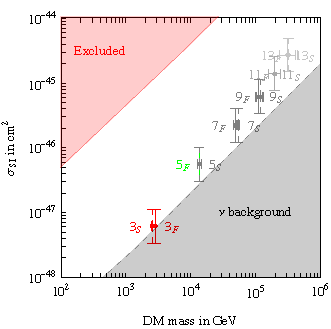
\includegraphics[width=0.3\textwidth,height=0.3\textwidth]{figs/MDMdirectPredictions} \qquad
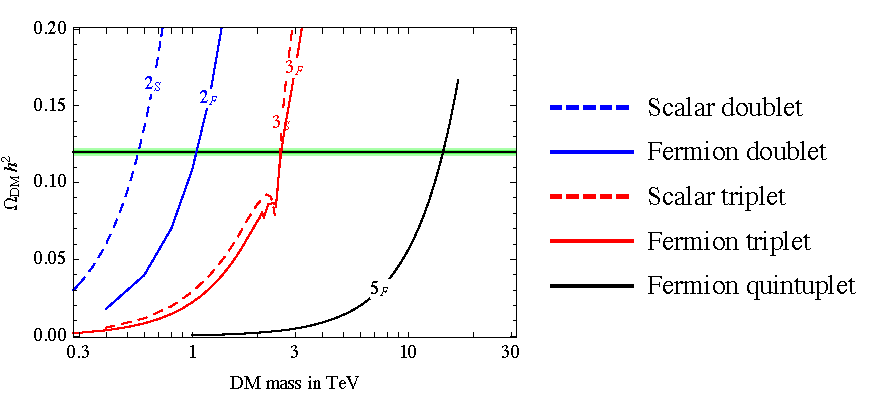
\includegraphics[width=0.63\textwidth,height=0.3\textwidth]{figs/OmegaMDM} 
\end{center}
\caption[Minimal Dark Matter mass]{\label{fig:MDMOmega}\em
Minimal Dark Matter in an $n$-plet representation of 
the $\SU(2)_L$ gauge group,
denoted as $n_{F,S}$, where  scalars ($S$) are dashed and fermions ($F$) continuous.
{\bfseries Left}: predictions for the mass and direct-detection cross section
(from \arxivref{2107.09688}{Bottaro et al.}~in~\cite{MDM}).
The mass predicted by freeze-out roughly scales as $n^{5/2}$ (having included Sommerfeld corrections);
$\sigma_{\rm SI}$ as $n^4$; indirect detection rates as $1/n^5$.
{\bfseries Right}: thermal DM abundance as a function of DM mass; 
the $3_F$ and $5_F$ curves include effects due to the bound states.}
\end{figure}



\subsubsection{Cosmological relic abundance of Minimal DM}\index{Minimal DM!cosmological abundance}\index{DM cosmological abundance!of Minimal DM}
DM annihilation cross section, relevant for thermal freeze-out, needs to be summed over all
quasi-degenerate Minimal DM components, in order to take co-annihilations into account.
The $s$-wave (co-)annihilation cross section at tree level, in the normalisation of section~\ref{chapter:indirect}, is given by
\begin{equation}\label{eq:MDMtree}
\sigma v_{\rm rel} =\left\{\begin{array}{ll}\displaystyle
\frac{g_2^4 (3-4n^2+n^4) + 16 Y^4 g_Y^4 + 8g_2^2 g_Y^2 Y^2 (n^2-1)}{128 \pi M^2 \, g_{\cal X}}
&\hbox{if ${\cal X}$ is a scalar,}\\[2mm]
\displaystyle
\frac{g_2^4 (2n^4+17n^2-19) + 4  Y^4 g_Y^2 (41+8Y^2)+16g_2^2 g_Y^2 Y^2 (n^2-1)}{256\pi\, M^2\, g_{\cal X}}
&\hbox{if ${\cal X}$ is a fermion,}
\end{array}\right.
 \end{equation}
where an $n$-plet of $\SU(2)_L$ has 
$g_{\cal X} = 2n$ degrees of freedom, if it is a complex scalar, while
$g_{\cal X}=n$ for a real scalar, and
 $g_{\cal X}=4n (2n)$ for a Dirac (Majorana) fermion.
Annihilations into SM fermions and Higgs are $p$-wave suppressed, if ${\cal X}$ is a scalar.

These expressions for the annihilation cross sections receive in the non-relativistic regime non-pertur\-bative corrections, if  $M \circa{>}M_W/\alpha_2$:
the Sommerfeld corrections and the bound-state formation (see section~\ref{Sommerfeld}).
Table~\ref{tab:MDM} lists for each choice of the Minimal DM multiplet the mass $M$ for which the cosmological DM abundance is reproduced, both 
in the tree-level approximation as well as when non-perturbative corrections are included. The required values of DM mass $M$ are in the TeV to multi-TeV range, somewhat above the reach of the present colliders.\footnote{
Minimal DM is the minimal realization of the\index{WIMP!miracle} `WIMP miracle', i.e., that thermal relic DM with weak interactions has a roughly weak scale mass, see sections~\ref{sec:WIMPs} and \ref{sec:thermalapprox}. 
In the past, the `WIMP miracle' was often understood as pointing to $M\approx 100\GeV $, as this resonated with the low energy supersymmetry hypothesis, which for such low WIMP mass would have also explained the small value of the Higgs mass, i.e., this would have been a natural solution to the hierarchy problem. 
MDM shows how in DM models with minimal extra content the `WIMP miracle' is actually realized for larger, multi-TeV, values of the DM mass. This is, in particular, a consequence of the larger size of the multiplets (co-annihilations are important and thus the cross section larger, see the high powers with which $n$ enters in eq.~(\ref{eq:MDMtree})) and of Sommerfeld and bound-state enhancements.}




\subsubsection{Indirect detection of Minimal DM}
The fermionic MDM candidates with $Y=0$ mainly annihilate  into $W^+W^-$ at tree level, while 
annihilations into $\gamma\gamma$ and $\gamma Z$ arise at 1 loop, see fig.~\ref{fig:MDMID}. 
Scalar MDM candidates can, in addition, also annihilate into pairs of Higgs bosons.

As for any other DM candidates, the annihilations of MDM particles result in various species of cosmic rays: $e^+$, $\bar p$, $\bar d$, $\gamma$. The phenomenology of thus generated charged cosmic rays follows the general discussion in section~\ref{sec:positronexcess}. 
The prompt gamma ray spectrum, however, is somewhat peculiar, since it features a prominent line at $E \simeq M$ in addition to a continuum shoulder at $E < M$. The latter is formed by $\gamma$-rays from the gauge bosons created in the final state parton showers. 
The  $\gamma$ ray peak at $E\simeq M$, on the other hand, is generated at 1-loop. In most models it is suppressed relative to the continuum contribution, but not in  Minimal DM.
This non-trivial result is a consequence of the Sommerfeld enhancement (see section~\ref{Sommerfeld}), which leads to comparable peak and continuum annihilation cross sections, for a range of DM masses. The formation and subsequent decay of bound states also has to be taken into account to properly compute the $\gamma$-ray spectrum.
 
The current status of the constraints for the most popular candidates (the {\em wino-like 3-plet} and {\em the Minimal DM 5-plet}) depends significantly on the assumed DM density profile in the Milky Way: if DM is cuspy in the center of the Galaxy, such candidates
 are ruled out across a large range of masses by {\sc Hess} and {\sc Fermi} limits, including the DM mass implied by the observed cosmological DM relic density. These models instead remain mostly viable if the DM density profile features a modestly-sized core. These conclusions seem to hold even after the refined, dedicated analyses performed in 2025~\cite{MDM}. 


In many DM models, DM particles that get captured in the Sun and then annihilate into neutrinos lead to important constraints, see section~\ref{sec:DMnu}. This is not the case for the Minimal DM models. Given the small values of the scattering cross sections on nuclei, in MDM models the capture in the Sun is very inefficient: the prospects for detecting a flux of high energy neutrinos from the Sun's core that would be due to MDM annihilations are bleak.

\begin{figure}[t]
\centering
$$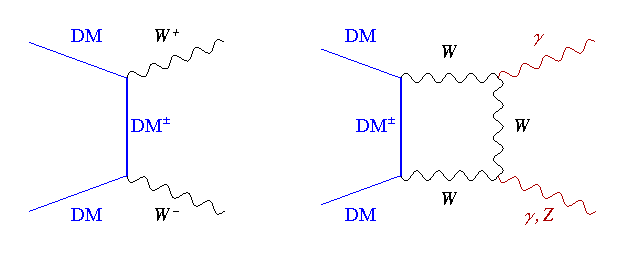
\includegraphics[width=0.6\textwidth]{figs/MDMindirectdetection} $$
\caption[Minimal Dark Matter indirect detection diagrams]{\label{fig:MDMID}\em Illustration of the main tree-level and 1-loop diagrams relevant for indirect detection of fermionic Minimal Dark Matter with $Y=0$.}
\end{figure}



\subsubsection{Collider searches for Minimal DM}
If the MDM particles are lighter than what is required to match the  observed cosmological  DM density via the minimal thermal freeze-out (that is, if cosmology is more complicated), then the MDM can be searched for at the LHC, via the standard signal channels: the mono-jet, the mono-photon, the vector boson fusion processes, and others (see section~\ref{chapter:collider}). A peculiarity of this class of models is the presence of slightly heavier charged states $\cal{X}^{\pm},\cal{X}^{\pm\pm}$. When the charged components of the MDM multiplet are produced in the LHC collisions, they decay into the neutral component and very soft charged pions, which are not reconstructed at the LHC. However, due to the smallness of the mass splitting, their lifetimes are relatively long; the corresponding decay lengths at rest are on the order of a few centimeters. A small but non-negligible fraction of the charged states, corresponding to the tail of the decay distribution, would therefore travel far enough to leave a track in the detector. These events would appear as high $p_T$ charged tracks that suddenly disappear inside the detector (the act of disappearing occurs when the charged state decays into DM and the unreconstructed $\pi^\pm$). 

Current searches at the LHC are sensitive at most to Minimal DM masses of a few hundred GeV.
MDM candidates provide, however, a well defined target for future colliders: the interactions of MDM are fully predicted by their quantum gauge numbers, 
while a thermal freeze-out  indicates multi-TeV values for their masses.
Disappearing charged tracks would provide maximal sensitivity, if these will be observable by tracker components of the future detectors.
In such an optimistic case, it is estimated that a futuristic 100 TeV $pp$ collider could directly probe 
a (Higgsino-like) fermion doublet  up to $\sim 1.5\TeV$,
a (Wino-like) fermion triplet  up to $\sim 6 \TeV$,
and a scalar triplet up to $\sim 3\TeV$, thereby covering the masses predicted by the thermal freeze-out~\cite{MDMcolliders}.
However, a fermion 5-plet would be probed only up to $\sim 6\TeV$, not covering the mass predicted by the thermal freeze-out. This unfortunately
provides a counter-example to the often repeated claim that a 100 TeV $pp$ collider can conclusively probe
weakly interacting dark-matter particles of thermal origin~\cite{GG}.
A futuristic muon collider could almost reach its kinematical limit $M \lesssim \sqrt{s}/2$, and could thus cover all MDM thermal targets for $\sqrt{s}\sim 30$\,TeV~\cite{MDMcolliders}.


\subsubsection{DM and neutrino masses}
Minimal DM candidates can be part of extended models that generate neutrino masses at one loop.
For example, a model is obtained adding to the SM the MDM fermion 5-plet  ${\cal X}$ with hyper-charge $Y=0$ and a
scalar 4-plet $S$ with  $Y=1/2$.
The resulting theory is invariant under ${\cal X}\to -{\cal X}$ and $S\to - S$
and contains a Yukawa coupling to leptons $L {\cal X} S$ and a $S^2 H^2$ quartic.
Together with the Majorana mass of ${\cal X}$, these interactions break lepton number.
Then, at one loop level ${\cal X}$ and $S$ mediate the Majorana neutrino mass operator $(LH)^2$~\cite{MDMnu}.



\subsection{Inert Higgs}\label{sec:inertHiggs}\index{Inert Higgs}\index{DM theory!inert Higgs}
The special case of an extra scalar doublet $H'$ with vanishing Yukawa couplings and a vanishing vacuum expectation value is known as  the {\em `inert Higgs'} or the {\em `Inert Doublet Model (IDM)'}~\cite{inertHiggs}.
In order to enforce the stability of the neutral component in $H'$, and thus a viable DM candidate, an unbroken $H'\to - H'$ symmetry is assumed (under which all the SM fields, including the usual SM higgs doublet, are even).
Particularly relevant is the quartic term $\lambda_5 \Re (H^* H')^2 $ in the scalar potential, which
splits the inert Higgs into its components,
$H'= (h^{\prime +}, (h' + i \eta')/\sqrt{2})$,
and qualitatively differentiates an Inert Higgs from a Minimal DM scalar doublet.
The DM candidate is the lightest neutral state, which is either the scalar $h'$ or the pseudo-scalar $\eta'$,
depending on the sign of the $\lambda_5$ coupling.
This mass splitting avoids exclusion from direct detection searches, because the $Z$-mediated scattering is now inelastic, see section \ref{sec:inelastic:DM:scattering}.
The Higgs-mediated scattering amplitude due to  $\lambda_5$ and other scalar couplings 
leads to small scattering rates, which are below the current constraints but can be searched for in the future. 
The DM cosmological abundance is reproduced via thermal freeze-out in two main distinct regions:
\begin{enumerate}
\item A `high mass' region around $M \sim 500\GeV$ where annihilations are dominantly into vector bosons,
like in the $\SU(2)_L$-invariant Minimal DM limit, see eq.\eq{MDMlagrangian}.
Thereby this region is the only one considered in table \ref{tab:MDM}.
\item Some `low-mass' islands around $M \sim70\GeV$, 
where the dominant DM annihilation process is mediated by the SM Higgs in the $s$-channel.
\end{enumerate}
Dedicated analyses find that even the second region is currently allowed by collider constraints.





\section{Models with dark forces and dark sectors}\label{sec:darksectors}
We now move to the scenarios in which DM is not charged under the known SM forces but rather charged under one or more hypothetical {\em dark force(s)}. 
The simplest possibility is a dark U(1) gauge symmetry. The associated dark gauge boson can be much lighter than the DM itself; it can even be massless and result in a long range dark interaction. 
The presence of a dark force changes significantly the phenomenology of dark matter. For instance, the DM\,DM annihilations in the presence of a long range dark force are Sommerfeld enhanced (see section~\ref{Sommerfeld}) and, in general, DM will be self-interacting (see section~\ref{sec:SIDM}).
In more general models, the DM particle could be accompanied by a whole ``dark sector'' of particles, possibly lighter than the DM itself. Such dark sectors can lead to a large set of possible signals that are accessible at energies within reach of laboratory experiments, see section~\ref{sec:searches:beam:dumps}.

That DM could be accompanied by a much larger dark sector should come as no surprise, as it would be reminiscent of the situation in the visible sector where the two stable matter particles, electron and proton, are accompanied by a much larger structure of elementary particles. Since the dark sector could be as complicated or even more complicated than the SM sector, it is next to impossible to cover all possible non-minimal models. One possibility is to focus on a particular complicated structure, hoping that this covers a large enough set of signatures. A popular choice is to postulate that the dark sector consists of one or more copies of the SM~\cite{MirrorSM}. This will be discussed in subsection~\ref{sec:dark:atoms}.
Another option is to considering dark sectors that are obtained by spontaneous breaking of a `unified' dark gauge symmetry, a possibility that we discuss in subsection~\ref{sec:DMSSB}.

\medskip

In the bulk of this section we follow a more minimal organizing principle, and assume that interactions between the SM and the dark sector 
can be well approximated as~\cite{Portals}
\beq
\label{eq:portal}
\bbox{\Lag_{\rm portal}=\sum_i c_i {\cal O}_{i\rm SM}  {\cal O}_{i\rm DS}}~,
\eeq
where ${\cal O}_{\rm SM}$ and ${\cal O}_{\rm DS}$ are local operators in the SM and dark sectors, respectively.
The most relevant {\em portal interactions} are those that are minimally suppressed by some high-energy scale.
Their structure depends on the unknown quantum numbers of dark sector particles,
usually dubbed a {\em ``dark Higgs''} or a {\em``light singlet''}, if the dark sector particle is a spin 0 scalar;
an {\em ``axion''} or {\em ``axion-like pseudo-scalar}, if it is a spin 0 pseudo-scalar;
a {\em ``dark photon''} or a {\em ``light $Z'$'',} if it is a spin 1 vector;
or  a {\em ``heavy neutral lepton''}, if it is a spin 1/2 fermion. 
At lowest mass dimensions of interactions, i.e., at dimensions 4 and 5, 
only a limited number of portals $\Lag_{\rm portal}$  can be written down. 
These are listed in table~\ref{tab:portals}. 
The dark photon, dark Higgs, and the neutral lepton portals are renormalizable, 
while the axion portal is suppressed by a high-energy scale represented by the axion decay constant, $f_a$, since it is assumed to be a pseudo-Nambu-Goldstone boson.

\medskip

In most dark sector constructions, and therefore also in this section, the common assumption is  that the dark sector particles discussed above
are merely mediators between the dark and visible sectors. 
The dark matter particle is usually assumed to be a different, additional state in the dark sector. 
However, a more minimal option is also possible --- the mediator itself, if sufficiently stable, can be the DM candidate, 
as long as it is produced in the correct amount to match the cosmological observations. 
Dark photon dark matter is briefly addressed at the end of subsection \ref{sec:VectorPortal} below, 
as well as in section \ref{GravDM}; axion-like particles as the DM are discussed in sections \ref{LightBosonDM} and \ref{axion}; heavy neutral lepton (a.k.a. sterile neutrino) as the DM is discussed in section \ref{FermionSinglet}; dark Higgs (scalar singlet) as a DM is discussed in section \ref{ScalarSinglet}.


\begin{table}[t]
\begin{center}
\begin{tabular}{lc}\normalsize
\\
\hline\hline
Portal & Interactions
\\[1mm]
\hline
Dark Photon, $A'_\mu \qquad$&  $-\epsilon F_{\mu\nu}'B^{\mu\nu}$
\\
Dark Higgs, $S \qquad$&  $(\mu S+\lambda S^2) H^\dagger H$
\\
Heavy Neutral Lepton, $N \qquad$&  $y_N L H N$
\\
Axion-like pseudo scalar, $a$ & $a F\tilde F/f_a$,  $a G\tilde G/f_a$, $ \big(\bar \psi \gamma^\mu \gamma_5 \psi\big) \partial_\mu a/f_a$
\\
\hline\hline
\end{tabular}
\end{center}
\vspace{-5mm}
\caption[Portals]{\em\label{tab:portals} The lowest dimension portals to the dark sector, 
and sketches of the corresponding interactions (see the main text for precise ${\mathcal O}(1)$ factors).}
\end{table}

\subsection{The vector portal}\label{sec:VectorPortal}\index{DM theory!portal!vector}\index{Mediators!vector}
The dark photon or vector portal couples the dark sector with the SM through a kinetic mixing term \cite{Dark:photon}, \index{Kinetic mixing}
\beq
\Lag_{\rm dark~photon}=\Lag_{\rm SM}+\Lag_{\rm DS}+\Lag_{\rm mix},\qquad
\Lag_{\rm mix}=-\frac{\epsilon}{2\cos\theta_{\rm W}} F_{\mu\nu}' B^{\mu\nu},
\eeq
where $B_{\mu\nu}=\partial_\mu B_\nu -\partial_\nu B_\mu$ and $F_{\mu\nu}'=\partial_\mu A_\nu'-\partial_\nu A_\mu'$ are the field strengths of the SM hypercharge, $\U(1)_Y$,  and the new dark $\U(1)'$, respectively.
The weak angle  $\theta_{\rm W}$ is kept in the definition of $\epsilon$ so that,
after the electroweak symmetry breaking, the kinetic mixing term becomes
\beq
\Lag_{\rm mix}=
\frac{1}{2}\epsilon F_{\mu\nu}'\big(F^{\mu\nu}-\tan\theta_{\rm W} Z^{\mu\nu}\big),
\eeq
where $F_{\mu\nu}$ ($Z_{\mu\nu}$) are the SM photon ($Z$) field strengths. 
The kinetic mixing parameter, $\epsilon$, is generated at least radiatively. 
If there are heavy fields charged under both $\U(1)_Y$ and $\U(1)'$,
the mixing is generated at 1-loop, $\epsilon \sim g_Y g_D/(4\pi)^2$. If not, the kinetic mixing is generated
at higher loops unless it is explicitly forbidden by a symmetry (see also the discussion in section~\ref{sec:milicharged}).

The dark photon Lagrangian may also contain 
a non-trivial dark sector with extra dark sector matter fields, $\chi$.
Assuming for concreteness that $\chi$ is a Dirac fermion we have
\beq
\label{eq:Lag:d:sec}
\Lag_{\rm DS}=-\frac{1}{4}\big(F_{\mu\nu}'\big)^2+\frac{1}{2}M_{A'}^2 \big(A_\mu'\big)^2+\bar\chi (i \partial_\mu- g_D A_\mu'\big)\gamma^\mu\chi- m_\chi \bar \chi \chi +\cdots.
\eeq
The dark fermion $\chi$ could be the DM, but does not have to be. 
The dark photon mass $M_{A'}$ is most often taken as a free parameter since only tree level effects are usually considered. If a UV complete model is needed, $M_{A'}$ can be assumed to come from spontaneous symmetry breaking, in which case $\Lag_{\rm DS}$ also contains a dark Higgs charged under $\U(1)'$. The dark Higgs obtains a vacuum expectation value, which then breaks the $\U(1)'$. 

\medskip

The dark photon phenomenology is most easily derived in a basis where the  quadratic part of the action is diagonal.
If the dark photon is massive, the mixing with the photon can be removed by a redefinition of the photon field
\beq
\label{eq:Amu:shift}
A_\mu\to A_\mu+\epsilon A_\mu',
\eeq
while the $A_\mu'$ field remains unchanged (and thus the $A'$ mass term is trivially still diagonal). 
As a consequence of the redefinition of eq.~\eqref{eq:Amu:shift}, the massive hidden photon couples to all electrically charged particles with the strength $\epsilon e$, and can be produced in the collisions of SM particles. 
At low energies the $Z$ boson  can be ignored.\footnote{Including the $Z$ boson in the diagonalization, the new interactions are up to ${\mathcal O}(\epsilon^2)$ given by the interaction Lagrangian
$- e \epsilon J^\mu A_\mu'+g_D \epsilon \tan \theta_{\rm W} J'{}^\mu Z_\mu +g_D J'{}^\mu A_\mu'$, where $J^\mu$ ($J'{}^\mu$) is the SM electromagnetic current (the dark current).}

\begin{figure}[t]
$$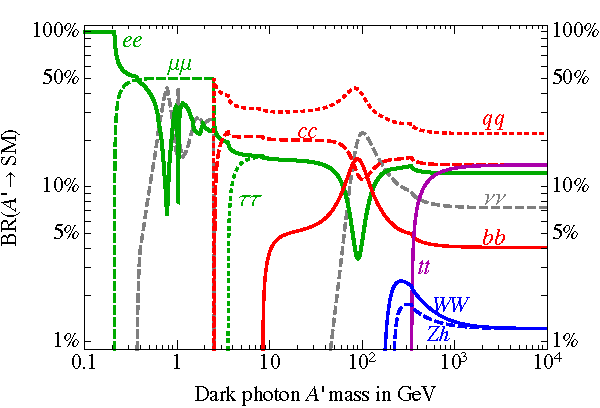
\includegraphics[width=0.55\textwidth]{figs/HiddenPhotonBR_new.pdf}$$
\caption[Dark Photon Branching ratio]{\em Predicted {\bfseries branching ratios for dark photon decays} with mass $M_{A'}$. 
The $A'\to e^+e^-$ decay mode (green solid curve) dominates below the  muon threshold, while above it 
${\rm BR}(A'\to \mu^+\mu^-)$  (green dashed) catches up. 
The decays into hadronic channels open around the $\pi^+\pi^-$ threshold. 
Between $350\MeV \lesssim M_{A'} \lesssim 2.5\GeV$ the hadronic resonances are approximated 
to decay half into $\mu^+\mu^-$ and half into $\nu\bar\nu$ 
(this approximation misses a small fraction of other SM particles, like photons from $\pi^0$ decays in the final state).
At $M_{A'}\gtrsim 2.5 \GeV$, the decay into quark pairs is perturbatively described and these channels pick up. 
At larger masses, different decay channels open at the relevant thresholds.
(Figure adapted from~\arxivref{1811.03608}{Sala et al.~(2018)}; see therein for details. For alternative presentations where the hadronic resonances are not decayed, see~\cite{DPBR}).
 \label{fig:DarkPhoton:Br}}
\end{figure}


\medskip

\index{Dark photon}
The phenomenology of the vector portal depends on the details of the dark sector. In the {\bf minimal dark photon model} the dark photon is assumed to be the lightest dark sector state, while the other dark sector particles are heavier and can be ignored. The phenomenology of the minimal dark photon model is controlled by only two parameters, $M_{A'}$ and $\epsilon$. 
If the dark photon is heavy enough, it decays back to the SM particles through the $- e \epsilon J^\mu A_\mu'$ interaction, leaving a visible imprint in the detector. 
All the relative branching ratios, $A'\to e^+e^-, \mu^+\mu^-, \pi^+\pi^-,$ etc., are fixed by the electro-magnetic current $J^\mu=- \big(\bar e \gamma^\mu e\big) +\tfrac{2}{3} \big(\bar u\gamma^\mu u\big)-\tfrac{1}{3} \big(\bar d\gamma^\mu d\big)+\cdots$, making the model predictive, see fig.~\ref{fig:DarkPhoton:Br}.\footnote{We acknowledge the help of F.~Sala for the figure.} 
A dark photon lighter than $2 m_e$ does not decay into visible SM states and instead appears as missing energy in the detector (such a light $A_\mu'$ does decay to SM neutrinos through one loop induced electroweak transition, with the neutrinos escaping the detector). 
A massless dark photon leads to the effects and constraints discussed around eq.\eq{sigmatran}.


A less minimal option is {\bf light dark matter coupled to dark photon}. The DM $\chi$ in eq.~\eqref{eq:Lag:d:sec} is then taken to be lighter than the dark photon so that the invisible decays $A'\to \chi \bar\chi$ are possible. In this non-minimal option the parameter space becomes larger, but still tractable, 
with four unknown parameters $\epsilon, g_D, M_{A'}, m_\chi$. 
For $g_D\gg \epsilon e$ the invisible decay channel dominates and the bounds on vector portal become much weaker, compared to the dark photon model. 

\smallskip

Finally, the {\bf millicharged particles} limit is obtained when $M_{A'}\to 0$ and both $\U(1)_{\rm em}$ and $\U(1)'$ are unbroken. The absence of vector masses allows to freely rotate the $A_\mu , A'_\mu$ fields.
This can be used to choose a basis more convenient than eq.\eq{Amu:shift},
imposing that SM charged particles
couple to one vector only, the photon.
The needed transformation is 
\beq
\label{eq:Amu:shift2}
A'_\mu\to A'_\mu-\epsilon A_\mu, \qquad A_\mu\to A_\mu,
\eeq
In this basis the DM $\chi$ carries a millicharge $|Q_\chi|\simeq|\epsilon g_D e|$ under the visible photon.\footnote{The physics of course does not depend on which basis is used
as long as both vector bosons are included in the calculations.  
For nonzero $M_{A'}$ the field redefinition eq.~\eqref{eq:Amu:shift2} does not keep the mass term diagonal, in contrast to~eq.\eq{Amu:shift}, making the latter a more convenient choice. 
The $M_{A'}\to 0$ limit is relevant when $q\gg M_{A'}$, where $q$ is the typical energy or momentum exchange in the process. 
For this to be valid in all observations, both at colliders 
($q$ from $\approx 0.1\GeV$ to $\approx\TeV$) and in astrophysics/cosmology, $M_{A'}$ needs to be very small, below $10^{-20}$ GeV.}
The general phenomenology of millicharged DM is discussed in section~\ref{sec:milicharged}.
\smallskip

More generally, if the SM fermions are charged directly under the $\U(1)'$, 
the dark photon is usually renamed as $Z'$. 
An example of such a $Z'$ is, for instance, the gauge boson of $\U(1)_{B-L}$ under which all the SM quarks carry a charge $+1/3$ and the SM leptons carry a charge $-1$ such that $\U(1)_{B-L}$  is anomaly free already just with the SM fermion content. Other options are possible, such as gauging the $L_\mu-L_\tau$ number, etc. The experimental bounds on dark photons or $Z'$s with general couplings can be obtained through the {\tt DarkCast} code~\cite{DarkCast}. 

The experimental constraints for the minimal dark photon model and for the dark matter coupled to a dark photon are shown in fig.~\ref{fig:dark:photon:constraints}.

\subsubsection{Dark Photon Dark Matter} 
As already mentioned above, the dark photon itself can be the dark matter~\cite{DPDM}.  
A number of different mechanisms for the production of the dark photon cosmological abundance have been considered in the literature, 
including the misalignment mechanism (see section~\ref{sec:misalignement})
as well as the inflationary production (section~\ref{sec:inflDMprod}). 
The plausible mass range for dark photon DM is wide, since it depends on the production mechanism. 
Typically, it extends from 1 MeV on the high end, down to the minimum DM mass value of about $10^{-21}$ eV 
(see eq.~(\ref{eq:DMmassrange})), although in specific models dark photon masses as large as $10^{14}$ GeV were also considered. 

The search strategies for dark photon dark matter are in broad strokes rather similar to the ones for the axion searches 
(though some of the techniques are specific to axions, see section~\ref{AxionExp}). 
For a detailed review of dark photon DM experimental searches and resulting constraints see \arxivref{2105.04565}{Caputo et al.~(2021)} in~\cite{DPDM}.



\subsection{The scalar portal}\index{DM theory!portal!scalar}\index{Mediators!scalar}
A scalar singlet $S$ can couple to the SM Higgs bilinear, $H^\dagger H$, forming the so called {\em scalar} or {\em Higgs portal} to the dark sector \cite{ScalarPortal}, 
\beq
\label{eq:scalar:portal}
\Lag_{\rm scalar}=\Lag_{\rm SM}+\Lag_{\rm DS}-\big(\mu S+\lambda_{SH} S^2) H^\dagger H,
\eeq
where $\mu$ ($\lambda_{SH}$) is a dimensionful (dimensionless) parameter. 
The set-up is very similar to that of scalar singlet DM (section \ref{sec:sterileDM}) except that here $S$ is the mediator rather than the DM candidate, and thus there is no requirement of a $Z_2$ symmetry that would stabilize $S$. 
The dark sector Lagrangian is 
\beq
\label{eq:LagDS:scalar:portal}
\Lag_{\rm DS}=\bar\chi (i \slashed{\partial}- m_\chi\big)\chi +\frac{1}{2}\big(\partial_\mu S\big)^2-\frac{1}{2}M_S^2 S^2+ y_\chi \bar \chi \chi S+\cdots,
\eeq
where for concreteness we again assume that $\chi$ is a Dirac fermion that may be the DM. 
After electroweak symmetry breaking, $H=(0, v+h/\sqrt{2})$ in the unitary gauge, 
the interaction term $\mu S H^\dagger H$ in \eqref{eq:scalar:portal} leads to the mixing between $S$ and the SM Higgs, $h$. The interactions of $S$ with the SM fields are induced through the mixing with the Higgs, and are thus the same as for the SM Higgs, except that they are suppressed by the mixing angle $\theta_S \simeq \mu v/(M_h^2-M_S^2)$. Phenomenologically important are the loop induced $b\to s S$ and $s\to d S$ decays, inducing the meson decays, $B\to K^{(*)} S$ and $K\to \pi S$, respectively. The quartic coupling $\lambda_{SH}$ gives rise to  $h\to SS$ decays, if $S$ is light enough, which can be a production channel of $S$ at the LHC. The singlet $S$ decays predominantly invisibly, if $2 m_\chi <M_S$ and $y_\chi \gg \theta_S y_f$  (with $y_f=m_f/v$ the Yukawa coupling of the heaviest SM fermion the $S$ can decay to). 


\subsection{The neutrino portal}\index{DM theory!portal!neutrino}\index{Mediators!neutrino}
The dark sector is assumed to contain {\em heavy neutral leptons} (HNLs), i.e.,\ gauge singlet fermions
here denoted as Weyl fermions $N_i$~\cite{NeutrinoPortal}. The HNLs are allowed by the SM gauge symmetry to have Yukawa interactions with the SM leptons, giving rise to the following portal\footnote{Here and elsewhere we use the compact notation $\bar N_i i \slashed \partial N_i= N_i^\dagger \bar \sigma^\mu i\partial_\mu N_i$ for Majorana fermion kinetic terms.} 
\beq
\label{eq:scalar:portalN}
\Lag_{\rm HNL}=\Lag_{\rm SM}+\bar N_i i \slashed \partial N_i - \left(\frac{M_{ij}}{2}N_i N_j  +y_{ai}\,    H \, N_i L_a + \hbox{h.c.}\right),
\eeq
where the summation over the SM lepton labels, $a=1,2,3$ and the HNL labels, $i=1,\ldots, n_N$, is understood. The dark sector Lagrangian 
contains mass terms for HNLs, with both Majorana and Dirac mass terms allowed. Since the motivation for HNLs mainly comes from neutrino mass models, the origin and structure of these mass terms may be of interest in itself. 

After electroweak symmetry breaking the Higgs obtains a vacuum expectation value, and the Yukawa interaction in eq.~\eqref{eq:scalar:portalN} mixes the SM neutrinos, $\nu_a$, with the HNLs, $N_i$, resulting in the mass eigenstates $\tilde \nu_a, \tilde N_i$. The net effect is that the interaction of HNLs with the SM are obtained by simply substituting in  $\Lag_{\rm SM}$ the SM neutrinos with $\nu_a=\tilde \nu_a+U_{ai}\tilde N_i$, where $U$ is the mixing matrix. In the minimal HNL models  both the production and the decays of HNLs are assumed to be fully determined by the mixing matrix elements $U_{ai}$ (in general, decays into the HNL sector may also be important). Very often an assumption of either electron, muon or tau dominance is made, i.e., that there is a single HNL, $N_1$, with only $U_{e1}$, $U_{\mu1}$ or $U_{\tau1}$ nonzero, respectively \cite{Portals}. The HNL mass is taken as a free parameter. 

Unlike the sterile neutrino DM case, discussed in section~\ref{FermionSinglet}, 
here there are no requirements for any of the HNLs to be the DM. 

\subsection{The pseudo-scalar portal}\index{DM theory!portal!pseudo-scalar}\index{Mediators!pseudo-scalar}\label{sec:ALP:portal}
The QCD axion is a light pseudo-scalar particle that is a pseudo Nambu-Goldstone boson (pNGB) arising from a spontaneous breaking of a global symmetry, solves the strong CP problem and is a viable dark matter candidate. The QCD axion is very light, with the axion mass  due entirely to the QCD anomaly, see section \ref{axion} for further details. 

The {\em axion like particle} (ALP) is instead a light pNGB that can be a viable DM candidate as a generalization of the QCD axion (see section \ref{LightBosonDM}) or can simply act as a mediator between the dark sector and the SM,\index{Axion-like particles} 
\beq
\Lag_{\rm ALP}=\Lag_{\rm SM}+\Lag_{\rm DS}+\frac{a}{f_a} \frac{\alpha_{\rm s}}{8\pi} G^a_{\mu\nu}\tilde G^{a\mu\nu}+ c_\gamma \frac{a}{f_a} \frac{\alpha}{8\pi} F_{\mu\nu}\tilde F^{\mu\nu} + \sum_\psi c_\psi \frac{\partial_\mu a}{f_a} \big(\bar \psi \gamma^\mu \gamma_5 \psi\big). 
\eeq
Here the sum runs over the SM fermions, both quarks and leptons, and we kept only the flavor diagonal couplings. The ALP couples to the SM fermions via a derivative coupling, since it is a PNGB, while the non-derivative couplings of ALP to gluons and photons arise when the spontaneously broken global symmetry is anomalous with respect to QCD and $\U(1)_{\rm em}$. The ALP mass, $m_a$, is taken to be a free parameter, and from the low energy perspective represents an explicit breaking of the shift symmetry $a\to a+\alpha$, where $\alpha$ is a phase. (Note that the coupling to gluons also contributes to ALP mass, $m_a$. For the QCD axion this is the only contribution, see eq. \eqref{eq:maxion} below).

\smallskip

The ALP parameter space is quite large. In addition to the ALP mass $m_a$, the coupling to gluons (given by $1/f_a$), and to photons ($c_\gamma/f_a$), there are also nine flavour-diagonal
couplings to quarks and charged leptons ($c_\psi/f_a$), as well as possible flavour-violating couplings.
Commonly used simplified benchmarks are: photon dominance (only $c_\gamma$ nonzero), gluon dominance (only the couplings to gluons are nonzero), or fermion dominance (taking for simplicity $c_\psi$ to be universal). This does give some estimate of how stringent the exclusions in the ALP parameter space are, but of course does not cover fully all the interesting possibilities. For instance, the flavor off-diagonal couplings to the SM fermions could well lead to the first observation of the ALP in the rare decays of $B, D$ or $K$ mesons \cite{FlavorViolatingALPs}. Note also, that the axion portal interactions are non-renormalizable.  Unlike the vector portal, the scalar portal and the neutrino portal, the axion portal thus requires a full high-energy theory, see section~\ref{AxionModels}. 
The ALP could be a DM: the case where this is a QCD axion is discussed further in section \ref{axion}.



\section{Composite Dark Matter}
\label{sec:compositeDM}
\index{Composite DM}
\index{DM theory!composite}
\index{DM properties!composite}
Quite generally, particles can be either elementary or composite, and this holds true also for DM. Composite particles are made out of elementary particles (scalars, fermions or vectors)\footnote{We do not
discuss in detail the AdS/CFT duality~\cite{AdS/CFT} as a tool
for approximating near-conformal strong interactions, via models in
warped extra dimensions, irrespectively of what the constituents are. 
For general discussion of extra dimensional DM models see section \ref{sec:Xdim}.}
 and can be strongly bound, like quarks and gluons inside a proton, or weakly bound, like proton and electron forming a hydrogen atom. 
 Typically, the compositeness scale $\Lambda$ corresponds to the inverse radius of the composite particle.
 Hence, at momentum exchanges smaller than $\Lambda$, and at energies smaller than the binding energy, composite DM appears as a point particle. 
This means that, for such low energies, our discussion so far, in which we treated DM as a point particle, still applies.  However, the renormalizable DM interactions get supplemented by additional 
non-renormalizable operators suppressed by the compositeness scale $\Lambda$ (sometimes these can be resummed into DM form factors, as was done for nuclear physics in the case of DM scattering on nuclei, see sections \ref{sec:SI} and \ref{sec:SD}, but now on the DM side). This means that, for precise phenomenology or for momentum exchanges above the compositeness scale, the composite nature of DM needs to be taken into account. 
If a DM signal will be observed in the future, one can try to measure these non-renormalizable interactions, and then use them  
to reverse-engineer the constituents and identify the right microscopic model.

The interplay between the compositeness scale and the constituents' mass also controls the DM mass. 
In strongly coupled theories when the masses of the constituents are smaller than the compositeness scale, then $M\approx \Lambda$. An example is the mass of a proton in the SM, which is comparable to the non-perturbative scale of QCD, $\Lambda_{\rm QCD}\approx 1\GeV$. 
If constituents are heavier than the compositeness scale, the DM mass is instead $M \gg \Lambda$. 
A SM example is the hydrogen atom, whose mass is to a good approximation given simply by the sum of the constituent masses, $m_{\rm H}\approx m_p+m_e$. This is much larger than the compositeness scale, corresponding in this case to the inverse Bohr radius, $1/a_0 = \alpha m_e$.

\medskip

At the moment, there are many possibilities for the models of composite DM. Dark sectors can  be quite complex in general, in the same way that the visible sector has a complex structure in the SM; with confining dynamics, long range forces, several stable states, etc. This means that, even in simple theories, stable dark relics could also follow a rather complex production history, quite different from the simplest thermal relic examples discussed in chapter \ref{chapter:production}. 
In fact, one can assume that the origin of dark matter may be linked to the origin of visible matter, i.e., 
that the generation of baryon asymmetry (the dominance of visible matter over antimatter) 
may be linked to the generation of dark baryon asymmetry. 
Composite DM models 
are therefore often also models of asymmetric DM.\footnote{
\index{Asymmetric DM!nuggets}
\index{Nuggets!asymmetric DM}
Such composite DM can also form {\bf asymmetric DM nuggets}, i.e.,~large composite states of $10^4$ or more asymmetric DM particles. 
Asymmetric DM models can lead to the formation of large bound states because they generically feature long-range attractive self-interactions due to a light mediator
(these are needed so that the annihilation rate is large enough that it efficiently depletes the symmetric component)~\cite{aDMnuggets}. 
This same mediator provides the attractive force that leads to nuggets. See also the discussion of quark nuggets in the SM, section \ref{sec:quarkmatter}.}
The latter is specifically discussed in sections \ref{sec:asymmetricDM} and \ref{sec:AsymmetricDMth}. 
In this section we focus on compositeness models  in general.
Such models can be divided into strongly coupled ones (section \ref{sec:strongly:coupled:DM:theories}) 
and weakly coupled ones (section \ref{sec:dark:atoms}).
We will discuss their main features, such as the possible patterns of symmetry breaking and their general phenomenology,
highlighting the differences with respect to elementary DM. 
A selection of  concrete models can be found in~\cite{BaryonicDM}. 


\subsection{QCD-like strongly coupled theories}\label{sec:strongly:coupled:DM:theories}
Arguably, the best understood strongly coupled theory is QCD, where we have at our disposal many experimental and theoretical insights. It is thus not surprising that the most studied models of composite DM are QCD-like. 
These models assume as matter content $N_F$ flavours of 
dark fermions $\Psi_i$, $i=1,\ldots, N_F$, that are in a vector-like representation of a `Dark Color' gauge group $\mathcal{G}_{\rm DC}$, either  $\SU(N)_{\rm DC}$, $\SO(N)_{\rm DC}$, or $\Sp(N)_{\rm DC}$, see table \ref{tab:chiralSB}.
Dark gauge interactions become non-perturbative at a scale $\Lambda$, resulting in a
 confinement of dark fermions and in the chiral symmetry breaking patterns listed in the second column of table \ref{tab:chiralSB}.
 
\smallskip
 
 Dark fermions $\Psi_i$ can in general be charged also under the SM gauge group, $\mathcal{G}_{\rm SM}$. The $N_F$ dark fermions are then organised into subsets, each of which belongs to a distinct irreducible representation of  $\mathcal{G}_{\rm SM}$ (some of the dark sector states will thus have a nonzero electric charge). Like in QCD, one can get a complex spectrum of composite states, starting from a simple microscopic Lagrangian with only a few free parameters. An appealing possibility is that, as in the SM, the strongly coupled dark sector also exhibits an accidental global symmetry,\footnote{A symmetry is {\em accidental} if it is not explicitly demanded in the construction of the renormalizable Lagrangian, but rather follows (at least in some limit)
from the assumed field content and their charges under gauge interactions. 
For example, baryon number and lepton number arise as accidental global symmetries 
in the renormalizable limit of the SM.} which then implies one or more stable composite particles, either dark baryons (composed of just $\Psi_i$) or dark pions (composed of $\Psi_i$ and $\bar\Psi_j$). 
These can be viable DM candidates, if they are electrically neutral, which can be the case even if they are composed of charged constituents, in the same way as the neutron in the SM is composed of charged quarks. 



\subsubsection{QCD-like dark baryons}\index{DM theory!composite!baryons}
An example of a theory where the DM consists of a dark baryon is a dark QCD with $N_F$
dark fermions in the fundamental representation of the Dark Color gauge group $\mathcal{G}={\rm SU}(N)_{\rm DC}$. 
The renormalizable Lagrangian of the theory is
\beq
\label{eq:Lag:dark:baryon}
\bbox{\begin{array}{rcl}
\Lag&=&\Lag_{\rm SM}+\bar \Psi_i \big(i \slashed D-m_i\big)\Psi_i -\frac{1}{4} G_{{\rm DC},\mu\nu}^a  G_{{\rm DC}}^{\mu\nu a} +\\
&&+\displaystyle \frac{g_{\rm DC} ^2 }{32 \pi^2}  \theta_{\rm DC} G_{{\rm DC},\mu\nu}^a  \tilde G_{{\rm DC}}^{\mu\nu a} +\big[ H \bar \Psi_i \big(y_{ij}^L P_L +y_{ij}^R P_R\big) \Psi_j+{\rm h.c.}\big]
\end{array}}
\eeq
where $G_{{\rm DC}}^{\mu\nu a}$ is the DC gauge field strength, and $g_{\rm DC}$ the corresponding gauge coupling. The Yukawa couplings $y_{ij}^{L,R}$ of DC fermions with the SM Higgs $H$ are nonzero only when they are allowed by the SM and dark gauge symmetries. 
This Lagrangian is accidentally invariant under a $\U(1)_{\rm DC}$ global symmetry, 
which rotates all the DC fermions $\Psi_i$ by the same phase, $\Psi_i \to e^{i\alpha} \Psi_i$. 
This guarantees the stability of the lightest dark baryon.\footnote{Like the SM baryon number, 
also the dark baryon number can be broken by weak anomalies.
Their effects are exponentially suppressed, 
so the lightest dark baryon can usually be treated as effectively stable for all practical purposes.}


In dark QCD the dark baryons are states composed of $N$ valence dark fermions, since these form a gauge invariant object when contracted with
the $\SU(N)_{\rm DC}$ anti-symmetric tensor.
For an even value of $N$ the dark baryons are bosons, while for an odd value of $N$ they are fermions, possibly with a large spin. 
If the lightest dark baryon, i.e., the DM candidate, is composed of electrically charged constituents, it
will have a large magnetic moment, in the same way as in the SM the  neutron has a large magnetic moment, even though it is electrically neutral. If DM has a large magnetic moment this could be resolved in direct detection experiments, since it would lead to a peculiar scattering pattern (both in terms of deposited energy and in the dependence of scattering rates on chosen target nucleus, see around eq.\eq{Q15}).

The masses $m_i$ of the dark  DC fermions $\Psi_i$ are free parameters. Just as in QCD, the dark constituents can be either lighter or heavier than the dark confining scale, $\Lambda_{\rm DC}$. 
As mentioned above, the two limits result in bound states with qualitatively different properties.
\begin{enumerate}
\item If constituents are lighter than $\Lambda_{\rm DC}$, then the DM properties are determined by the non-perturbative regime of the $\SU(N)_{\rm DC}$: DM has a mass $M \approx \Lambda_{\rm DC}$,
spatial size $1/\Lambda_{\rm DC}$, and
a non-perturbative annihilation cross section $\sigma \approx 1/\Lambda_{\rm DC}^2$. 
In this case, the
thermal relic abundance is reproduced for $M \approx100\TeV$, i.e., saturating eq.\eq{100TeV}.\footnote{If the dark QCD phase transition is first order and/or if the model is non-minimal with light degrees of freedom that decay slowly, the expected value for $M$ can be even multi PeV \cite{1912.02830}.}

\item
If, on the other hand, {\em all the dark constituents have a mass $m_i$  above $\Lambda_{\rm DC}$}, then the relevant $\SU(N)_{\rm DC}$ dynamics is perturbative. 
In this case DM is composed only of the lightest such constituents (of mass $m$).
The DM in this case behaves as a perturbative bound state
(similar to hadrons made of heavy $c,b$ quarks in QCD):
the DM mass is $M\approx N m$, 
and the annihilation cross section is set by its
Bohr-like radius $1/m\alpha_{\rm DC}$.
\end{enumerate}
Similar conclusions can be reached for the $\SO(N)_{\rm DC}$ and $\Sp(N)_{\rm DC}$ dark gauge groups. In the ${\rm SO}(N)_{\rm DC}$ models the dark baryons composed from $N$ fermions do exist and are also stable, thanks to a $\mathbb{Z}_2$ symmetry.
Among others, this means that two dark baryons can now annihilate.
In models with the $\mathcal{G}={\rm Sp}(N)_{\rm DC}$ gauge group, on the other hand, it is possible to have stable dark meso-baryons
composed out of two dark fermions
(mesons and baryons are the same object for ${\rm Sp}(N)_{\rm DC}$).


\begin{table}[t]
$$\begin{array}{c|cc}
\hbox{Gauge group $\mathcal{G}$} & \hbox{Fermion symmetries $\mathcal{G}_F\to \mathcal{H}_F$}   &\hbox{Scalar symmetries} \\ \hline
\SU(N)_{\rm DC} & \SU(N_F)_L\otimes \SU(N_F)_R\to \SU(N_F) &{\rm U}(N_S)  \\
\SO(N)_{\rm DC} & \SU(N_F) \to \SO(N_F) &  \mathrm{O}(N_S) \\
\Sp(N)_{\rm DC} & \SU(N_F)\to \Sp(N_F) & \Sp(2 N_S) 
\end{array}$$
\caption[Patterns of chiral symmetry breaking]{\em\label{tab:chiralSB}  
Assuming the confining dark gauge groups listed in the first column, we show in the second column 
the patterns of chiral symmetry breaking induced by condensates of
$N_F$ light fermions in the fundamental representation.
In the third column we show the symmetry associated to $N_S$ light scalars in the fundamental.
It can be broken by condensates or vacuum expectation values in different ways. 
See, e.g.~\cite{CompositeHiggsDM} for extra details. 
}
\end{table}




\subsubsection{Dark glue-balls}\index{DM theory!composite!glue-balls} \label{sec:darkglueballs}
The scenario discussed at point 2.\ above --- a dark gauge group $\mathcal{G}$ with all fermions or scalars heavier than its confinement scale
$\Lambda_{\rm DC}$ --- predicts, in addition to heavy dark baryons as DM candidates,
the possible existence of dark glue-balls with mass $M_{\rm DG} \sim \hbox{few}\, \Lambda_{\rm DC}$. These are bound states consisting of (dark) gauge bosons alone. As DM candidates, they are typically unfit because they are unstable.
In addition, they can be long-lived enough that they become problematic in the cosmological context. 
On the other hand, their small mass makes them a good target in the context of searches of dark sector states at colliders or accelerators.

For example, the lightest glue-ball is likely the state corresponding to the gauge-invariant operator
$\Tr {\cal G}^2$, with quantum numbers
$J^{CP} = 0^{++}$, meaning that it can be thought as a two dark-gluon state (${\cal G}$ is the matrix of dark gauge vectors in the adjoint representation of $\mathcal{G}$).

In the presence of heavy fermions or scalars charged under both $\mathcal{G}$ and $\mathcal{G}_{\rm SM}$,
two dark-gluons can annihilate into SM vectors $VV$ (gluons or electro-weak).
This means that the dark-glue-ball decays into $VV$ via the dimension-8 operator
$ \sim \alpha_{\rm D}\alpha_{\rm SM}\, \Tr G^2 \, \Tr V^2/M^4$, with rate
\beq \Gamma_{\rm DG} \sim \frac{\alpha_{\rm D}^2 \alpha_{\rm SM}^2 \Lambda_{\rm DC}^9}{4\pi M^8}.\eeq
If $M \gtrsim 10^3 \Lambda_{\rm DC}$ the dark glue-ball life-time exceeds one second and conflicts
with Big Bang Nucleosynthesis bounds.
Dark glue-balls can also decay faster, via the dimension-6 $(\Tr  G)^2 |H|^2$ operator,
in models where dark quarks have Yukawa couplings to the Higgs doublet $H$.
In an effective field theory context below the weak scale one can also have dimension-7 $(\Tr G)^2 f \bar f$ operators
involving SM fermions $f$.


In the absence of any additional matter content, the dark sector has no renormalizable interactions with the SM.
The lightest dark glue-ball can thus decays only gravitationally (see section \ref{GravDM}), with slow rate $\Gamma \sim M^5/M_{\rm Pl}^4$ and therefore is an acceptable DM candidate with life-time $\tau\gtrsim10^{26}\,{\rm sec}$ (see section~\ref{chapter:indirect}) if $M\circa{<} 100\TeV$~\cite{GravDM}.
Depending on the dark gauge group $\mathcal{G}$, other dark states beyond the lightest glue-ball may be metastable
in view of a C-parity and/or a P-parity in the dark gauge group.
These parities are discussed in general in section~\ref{sec:accidentallystable}, and we here summarise their implications for glue-balls.
If the dark gauge group is $\mathcal{G}=\SU(N)$, the spectrum contains C-odd glue-balls that correspond to the operator $\Tr G\{G,G\}$.
The lightest of these is gravitationally stable and decays with a highly suppressed rate $\Gamma\sim M (M/M_{\rm Pl})^8$, induced by possible  non-renormalizable operators that break the dark C-parity. 
The $\mathcal{G}=\SO(N)$ theories with $N\ge 6$, and $N$ even, contain glue-balls 
odd under a parity P in the dark group 
and corresponding to the operators ${\rm Pf}\,{\cal G}$.
The lightest of these is also gravitationally stable and decays only in the presence of  non-renormalizable operators that break dark P-parity, leading to the highly suppressed decay rate $\Gamma\sim M (M/M_{\rm Pl})^{2N-4}$. 
P-odd glue-balls therefore constitute acceptable gravitational DM candidates even for very large values of $M$ (for reasonably large $N$). 





\subsubsection{QCD-like dark pions}\label{sec:darkpi}\index{DM theory!composite!pions}
If $N_F$ dark fermions are lighter than $\Lambda_{\rm DC}$ then the dark sector Lagrangian satisfies an approximate accidental global symmetry $\mathcal{G}_F$. For instance, in dark QCD this is $\mathcal{G}_F=\SU(N_F)_L\otimes \SU(N_F)_R$ under which the dark fermions transform as $\Psi_{L/R,i} \to [\exp(i \alpha_{L/R}^a T^a)]_{ij} \Psi_{L/R,j}$, with $T^a$ the generators of $\SU(N_F)$ in the fundamental representation and $\alpha_{L,R}^a$ free parameters (the symmetry is exact in the limit $m_i\to 0$).
The dark fermion condensates break $\mathcal{G}_F$ to its subgroup $\mathcal{H}_F$ as listed in table~\ref{tab:chiralSB}.\footnote{Note that some works study effective field theories of composite dark particles  assuming  arbitrary $\mathcal{G}_F$ and $\mathcal{H}_F$ without discussing how such breaking patterns are achieved from microscopic dynamics of constituents. It is far from clear that such general symmetry breaking patterns can in fact be realized. } The symmetry breaking condensates are either 
$\med{\Psi\bar\Psi}\ne 0$, in the case that the dark fermions are in a complex representation, e.g., in the fundamental of
$\mathcal{G}={\rm SU}(N)_{\rm DC}$, or they can be $\med{\Psi\Psi}\ne 0$, e.g., for dark fermions that are in the 
fundamental representation of
${\rm SO}(N)_{\rm DC}$ or ${\rm Sp}(N)_{\rm DC}$.

 
The spontaneous breaking of a global symmetry implies the existence of pseudo-Nambu-Goldstone bosons (pNGB) --- pion-like scalar bound states lighter than $\Lambda_{\rm DC}$ --- which parametrise the $\mathcal{G}_F/\mathcal{H}_F$ coset. The existence of dark pions is phenomenologically important. 

First of all, even for models in which the DM candidate is a dark baryon, 
the first collider signatures of such models could be the production of dark pions rather than DM. 
Dark pions are normally lighter than dark baryons, and thus easier to produce. 
In general, they are also unstable, since they can decay into SM vectors through anomalies, 
and are thus easier to observe.

\smallskip

Secondly, if the dark sector Lagrangian is invariant under additional symmetries, some of the {\em dark pions can actually be stable and be DM candidates}.
A common possibility for such an additional symmetry are the dark species numbers. 
These arise if dark fermions $\Psi_i$ belong to two or more irreducible representations of the SM gauge group 
(that is, if dark sector is composed of several different species  of dark fermions, $\Psi_a$, each furnishing a different irreducible representation of the SM gauge group, while being in the same representation of $\SU(N)_{\rm DC}$). 
Depending on the full field content of the theory, the phase rotations acting individually on each representation $\Psi_a$ may be an accidental  `dark-flavor' symmetry. 
For instance, in the dark QCD Lagrangian of eq.~\eqref{eq:Lag:dark:baryon} 
the dark species number is an accidental symmetry for all dark species for which 
the Yukawa couplings vanish, $y_{aj}^{L,R}=0$.
Dark pions composed of different species of dark fermions, $\pi_{ab}\sim \bar{\Psi}_a \Psi_b$, are then stable, 
at least as far as renormalizable interactions are concerned.
Heavy UV physics can alter these conclusions. 
In many models, such flavour symmetries are explicitly broken by 
 dimension-5 or dimension-6 operators, which then lead to too fast decays of dark pions for these to be considered viable DM candidates. 

\smallskip

It is also possible to have accidental symmetries that are of group-theoretical nature.
For example, some models exhibit a symmetry analogous to the $G$-parity in QCD,
$\Psi_i \to [\exp(i \pi T^2)]_{ij}\Psi_j$, leading to a stable lightest dark-pion that can be a DM candidate~\cite{BaryonicDM}.
This happens in models with the
$\SU(N)_{\rm DC}$ gauge interaction that have $N_F=3$ dark fermions 
in the  triplet (real) representation of the electroweak $\SU(2)_L$ gauge group.
The $\SU(N_F)_L\otimes \SU(N_F)_R\to \SU(N_F)$ spontaneous breaking of the  flavor groups results in $N_F^2-1$ pseudo-Goldstone bosons that form a $3\oplus 5$ representation of $\SU(2)_L$.
 Because of $G$-parity, the triplet pNGB is stable and has the phenomenology of the Minimal Dark Matter scalar triplet, see section \ref{MDM}.


If DM is a dark pion, this has other phenomenologically interesting consequences. 
For example, various strongly interacting theories allow for interactions involving an odd number of dark pions.
such as the  Wess-Zumino-Witten interaction among 5 dark pions.
The resulting DM DM DM $\leftrightarrow$ DM DM scattering at nearly strong coupling
realises the scenario for a sub-GeV thermal relic DM discussed in section~\ref{sec:3<->2eq}~\cite{MeVDM}.



\subsection{QCD-unlike strongly coupled theories}
While dark QCD may be a useful benchmark model for composite DM, it by no means exhausts all the possibilities. 
Other possibilities include:
\begin{itemize}
\item[\scalebox{0.6}{$\blacksquare$}] 
Some strongly coupled gauge theories with vector-like fermions result in
{\bf confinement without chiral symmetry breaking}, corresponding to vanishing fermions condensates.
This new phenomenon was proven in some supersymmetric theories.
A non-supersymmetric example might be $\SU(N)$ with 3 fermions in the adjoint~\cite{anomaly:matching}.
In these models, dark-colored fermions much lighter than the confinement scale must
form composite fermions much lighter than the confinement scale, $M \ll \Lambda_{\rm DC}$, 
as demanded by 't Hooft anomaly matching conditions~\cite{anomaly:matching}.
Such composite dark baryons might be accidentally meta-stable DM candidates, and would behave as 
elementary particles up to corrections of order $M/\Lambda_{\rm DC}$~\cite{anomaly:matching},
differentiating them from QCD-like baryons such as the proton.


\item[\scalebox{0.6}{$\blacksquare$}]

Dark sector with gauge interactions but with matter content composed of {\bf massless chiral fermions} is another possibility~\cite{ChiralCompositeDM}.
This is theoretically appealing, since all scale(s)
$\Lambda_{\rm DC}$ are generated by dimensional transmutation.
DM can similarly be dark protons or dark pions.
These models tend to employ multiple gauge groups in order to avoid gauge anomalies,
for example mimicking a chiral family of the SM by postulating extra $\U(1)\otimes \SU(2)\otimes\SU(3)$ dark groups,
or partially employing the factors of the SM gauge group.
Multiple gauge groups allow to get chirality from a weakly coupled factor, 
avoiding the poorly known dynamics of strongly coupled chiral theories.\footnote{In chiral theories, the QCD-like scalar condensates of two fermions $\langle \bar\Psi\Psi\rangle$
are forbidden by gauge invariance
(because, if $\bar\Psi \Psi$ were allowed, one could add mass terms to fermions, and the theory would not be chiral).
So strongly-coupled chiral gauge theories could either form no condensates,
or form vector condensates $\langle \bar\Psi\gamma_\mu\Psi \rangle\ne 0$.
In such a case  the Lorentz group would be broken spontaneously in the dark sector ---
a possibility disfavoured by the smallness of the cosmological constant and by bounds on Lorentz symmetry breaking.}
The more complicated chiral models can lead to dark pions as the DM, with the DM decay rates more suppressed
than in the simple vector-like models.

\item[\scalebox{0.6}{$\blacksquare$}]
The matter content in the dark sector could be composed of {\bf dark scalars} instead of dark fermions, or one could have both dark scalars and dark fermions.
This more general field content then allows to build explicit models where both DM and the Higgs are composite~\cite{CompositeHiggsDM}.
However, less is known about strong gauge dynamics of scalars. The last column in table~\ref{tab:chiralSB} shows, for each gauge group class, 
the global flavor symmetries for models containing $N_S$ scalars, assuming these are unbroken. 
In explicit models the flavor symmetries can be broken, with the symmetry breaking pattern being model-dependent.


\item[\scalebox{0.6}{$\blacksquare$}]
One can consider theories where, instead of gauge interactions becoming non-perturbative, the strong coupling is either a {\bf Yukawa interaction} or {\bf scalar quartics}.  
\end{itemize}

\subsection{Weakly-coupled bound states: dark atoms and mirror DM}

\label{sec:dark:atoms}
Even if the interactions in the dark sector are perturbative, dark matter particles can still form (weakly) bound dark states. These can be unstable, for instance if they are formed from DM and its antiparticle \cite{BoundStates}, akin to quarkonia in QCD, or can be stable, if they are formed from two different species of DM particles. The formation of unstable bounds states, whose constituents eventually annihilate, can be an important effect in the early Universe and can change significantly the predicted relic abundance. They were discussed, together with Sommerfeld corrections, in section \ref{Sommerfeld}. Stable bound states, instead, are the so called {\bf dark atoms} \cite{dark:atoms} \index{DM theory!dark atoms}\index{DM theory!composite!dark atoms}\index{Dark!atoms}and we focus on them in the following. 

\bigskip

The simplest example of a dark sector in which dark atoms form is a model with two species of dark fermions, a dark proton and a dark electron, that carry opposite charges under a hidden $\U(1)_{\rm D}$ gauge symmetry, 
\beq
\label{eq:Lag:dark:atom}
\Lag_{\rm D}=\bar \Psi_{{\rm D}p}\big(i\slashed D+m_{{\rm D}p}\big)\Psi_{{\rm D}p}+\bar \Psi_{{\rm D}e}\big(i\slashed D+m_{{\rm D}e}\big)\Psi_{{\rm D}e},
\eeq
with $D_\mu=\partial_\mu+ i g_{\rm D} Q_{\rm D} A_\mu^{\rm D}$, and $Q_{\rm D}=\pm1$ 
for dark proton and electron, respectively. 
This model has three parameters, the dark gauge coupling constant, $g_{\rm D}$, 
and the masses of dark proton and electron, $m_{{\rm D}p}$, $m_{{\rm D}e}$ (without loss of generality one can define the dark proton such that, $m_{{\rm D}p}> m_{{\rm D}e}$). 
The formation of dark atoms is one of those cases in which the existence of an asymmetry in the dark sector is typically required, i.e.~a relic abundance of dark protons and dark electrons without dark anti-protons and anti-electrons, analogous to what occurs in the SM sector.

\smallskip

Due to the presence of dark atoms, the cosmological evolution is richer than in the case of a single elementary DM species. 
In general, the dark sector temperature $T^\prime$ will differ from the temperature $T$ in the visible sector. Furthermore, the ratio $T'/T$ can change during the evolution of the Universe, following different entropy injections in the two sectors. If the dark photon is massless, its two degrees of freedom account for an extra contribution to the relativistic energy density $\Delta N_{\rm eff} = 8/7 \, (11/4)^{4/3}\, (T^\prime/T)^4$ (see eq.~(\ref{eq:DeltaNeff}) in App.~\ref{sec:app:particles:thermal}). The current rather loose bound $\Delta N_{\rm eff} < 0.33$ at 2$\sigma$ \cite{Planckresults} implies the not very stringent constraint $T^\prime < 0.55 \, T$.
In dark atom models the dark sector interactions can decouple much later than in the conventional cold DM models with elementary DM particles. This has implications for structure formation: for instance, the proto-halo formation can be suppressed for proto-halos with masses below $\sim 10^3-10^6 M_{\odot}$. An important aspect of dark atom models is that now DM is a mixture of neutral and ionised components. The ionized fraction is phenomenologically important since it interacts through a long range force: bounds on self-interactions of DM (see section \ref{sec:SIDM}) are an important constraint. 
The self-interactions lead to energy dissipation (the same as electromagnetic interactions do for visible baryons), which then in general leads to denser, cuspier DM profiles~\cite{dark:atoms}. Another potential effect of dissipation is that (a subdominant component of) atomic DM can form many intermediate-mass black holes that act as seeds for the otherwise puzzling existence of early massive BHs~\cite{dark:atoms}. 

Assuming interactions with the visible sector, these lead to scattering in direct detection experiments as for usual cold DM. The difference with the elementary DM is that the scattering of dark atoms can result in outgoing dark atoms in an excited state: if these are short-lived they can result in additional signatures in the detectors, if the decays to visible sector particle are frequent enough. 

Within the dark atom hypothesis it is quite natural to entertain also the existence of dark molecules, dark compounds, and an entire {\em dark chemistry}. A few recent works have started exploring the implications of these concepts, especially in star formation and the early Universe evolution~\cite{dark:atoms}.



\bigskip

\index{DM theory!mirror DM} \index{Mirror world}
\label{sec:mirror:DM}
The special case in which the free parameters of the dark atoms ($g_{\rm D}$, $m_{{\rm D}p}$ and $m_{{\rm D}e}$) coincide with the values in the visible sector is called  {\em mirror world}~\cite{MirrorSM}. 
In this setup, the entire SM has a mirror copy, including quarks and leptons and force mediators. In particular, the baryons of the mirror sector are, like the visible ones, stable particles; they interact with mirror photons but they are dark in terms of the ordinary photons. 
Hence they could constitute a DM candidate known as the {\bf mirror DM}. 


The two sectors communicate via gravity but also via the mixing of the neutral SM and mirror particles: photons, neutrons, neutrinos.
The latter two mixings can give rise to co-baryogenesis/leptogenesis, inducing comparable baryon asymmetries and hence $\Omega_{\rm DM}\sim \Omega_b$.
The mirror symmetry cannot however be exact and, in particular, the mirror sector needs to have a lower temperature in order to agree with cosmology, including cold mirror DM, as discussed above. This can be realized if the two systems are born with different temperatures at reheating.
 
Besides providing mirror DM, the mirror world theory also makes several specific cosmological and astrophysical predictions. 
Mirror BBN would lead to a higher fraction of mirror He, so that mirror stars would be bigger, possibly seeding the observed
ultra-heavy black holes. The bullet cluster bound (see section \ref{sec:bullet}) can be satisfied if at least half of the mirror sector DM is in dark stars, rather than in gas.
If the baryon asymmetries have opposite sign, $\bar n \leftrightarrow  n'$ oscillations would allow appearance of $\bar n$
out of the mirror sector (for example in neutron stars), possibly allowing to explain the anti-matter events claimed by AMS (section~\ref{sec:antiHeexcess}) and providing a connection with the neutron decay anomaly (section \ref{neutrontau}).

\bigskip

Before concluding this section, we mention the proposal of \index{DM theory!composite!O-helium DM} {\bf O-helium}~\cite{Ohelium}, a model that is sometimes referred to as `dark atom' but is actually a hybrid of the strongly-coupled DM described in section \ref{sec:strongly:coupled:DM:theories} and the atomic physics discussed here. 
In this model, a techni-color-like or a QCD-like theory leaves stable, massive (typically $M \sim$ TeV), doubly charged O$^{--}$ particles that then bind to He$^{++}$ nuclei just after nucleosynthesis. The exotic O$^{--}$He$^{++}$ `atom' may constitute the DM and may be searched for with the techniques discussed in section~\ref{sec:SIMP}.
 





\section{Dark magnetic monopoles}
\label{Dmonopoles}
\index{Monopole}
\index{DM theory!monopole}

Quantum field theory predicts a variety of topological defects that can arise
when a gauge symmetry group $\mathcal{G}$ is spontaneously broken to its sub-group $\mathcal{H}$. 
An example are magnetic monopoles~\cite{magnetic:monopoles}, particle-like configurations of gauge and scalar fields  concentrated around a point in space, which are made stable by topology when the second homotopy group
$\pi_2(\mathcal{G}/\mathcal{H})\neq 0$ is non-trivial \cite{topological:defects:books}.
Loosely speaking, this means that there exists a mapping of a sphere in physical space (the boundary of 3-dimensional space at infinity)
into a sphere in the coset $\mathcal{G}/\mathcal{H}$, which cannot be continuously shrunk to a single point in $\mathcal{G}/\mathcal{H}$.\footnote{More concretely, consider a scalar field  $\varphi$ in some representation of group $\mathcal{G}$. 
Its expectation value results in $\mathcal{G}\to \mathcal{H}$ spontaneous symmetry breaking. 
A magnetic monopole corresponds to a topologically stable configuration of $\varphi$ of finite energy. 
For this to be the case the scalar potential needs to vanish far from the origin, 
$\lim_{|\vec x|\to \infty}V(\varphi (\vec x))=0$, 
while the value of $\lim_{|\vec x|\to \infty} \varphi (\vec{x}) \equiv  \varphi (\hat{\vec{x}}) $ is nonzero, 
and is different in different directions $\hat{\vec{x}}$. 
With a particular $\varphi(\vec x)$ configuration there is also an associated configuration of unbroken gauge fields, 
which then define the magnetic monopole. 
Since $\varphi$ does not change under $H$, the values $\varphi(\hat{\vec{x}})$ live in the $\mathcal{G}/\mathcal{H}$ coset, 
and give the mapping of the space boundary,  the two-dimensional sphere $S_2$, into the $\mathcal{G}/\mathcal{H}$ coset. 
If this mapping is topologically nontrivial, i.e., there is no continuous deformation that can make $\varphi(\hat{\vec{x}})$ vanish while keeping $V(\varphi (\hat x))=0$, the configuration is stable. 
This is possible only, if $\pi_2(\mathcal{G}/\mathcal{H})\neq 0$. 
For example, for any simply connected Lie group $\mathcal{G}$ broken to $\mathcal{H}$ one has $\pi_2(\mathcal{G}/\mathcal{H})=\pi_1(\mathcal{H})$, so that there are monopoles, if the first homotopy group of the unbroken subgroup is nontrivial, i.e.,  there are nontrivial mappings of a circle into $\mathcal{H}$. 
This is, for instance, the case for $\mathcal{H}=\U(1)$, for which $\pi_2(\mathcal{G}/\U(1))=\pi_1(\U(1))=\mathbb{Z}$, 
i.e., there is a discrete number of monopoles that carry integer magnetic charges $k$.}
Since it is impossible to unravel a topologically nontrivial configuration  in $\mathcal{G}/\mathcal{H}$,  the magnetic monopole is stable, which is a good start to be considered as a DM candidate.


\medskip

As anticipated in section~\ref{EWboundtstates}, 
the SM electro-weak phase transition does not lead to monopoles, 
since the associated second homotopy group is trivial, $\pi_2(\SU(2))=0$.
We then need to consider new-physics models~\cite{DarkMonopoles}.
Let us focus on the simplest possibility, $\mathcal{H}=\U(1)$. This $\U(1)$ cannot be the usual electro-magnetism, 
since electro-magnetic monopoles  are subject to strong experimental bounds ---
DM cannot be a magnetic monopole of the usual electro-magnetism. 
The simplest example of a theory with a dark sector magnetic monopole is thus 
 a dark $\mathcal{G}=\SU(2)$ gauge group with a scalar $S$ in the adjoint  representation. The dark   $\SU(2)$ is spontaneously broken to its $\U(1)$ subgroup once $S$ obtains a vacuum expectation value, 
$\langle S\rangle =w\,\diag(1,-1)/2$ (\arxivref{1406.2291}{Khoze and Ro (2014)} in~\cite{DarkMonopoles}).
At the perturbative level, the spectrum contains a  massive Higgs-like scalar (neutral under the dark $\U(1)$),
a massless dark photon $A'$,\footnote{Massless vectors result in extra dark radiation in cosmology.
Current bounds are satisfied, if the dark sector decouples from the SM
early enough (say, before the QCD phase transition), 
and is thus  significantly colder than the SM plasma at later stages of the cosmological evolution.}
and massive charged vectors $V^\pm$ (charged under  dark $\U(1)$). 
The charged vectors have mass $M_V =gw$, carry a charge $g$ under the dark $\U(1)$, 
are stable and are thus good DM candidates ($g$ is the dark gauge coupling).
The non-perturbative spectrum contains
magnetic monopoles which have a mass $M =4\pi w/g$ (up to corrections from possible non-vanishing scalar quartics).
The magnetic monopoles carry a magnetic charge $g_{\rm mag}=4\pi/g$ under the dark $\U(1)$, are stable, 
and are also viable DM candidates. 

The monopoles are produced during the
$\mathcal{G}\to \mathcal{H}$ phase transition which occurs at temperature $T \sim M_V$. 
The production rate depends on the nature of the phase transitions,
see section~\ref{DmonopolesKZ} for details. 
In particular, for this simplest model under consideration, the dark monopoles can constitute an ${\mathcal O}(1)$ fraction of DM relic abundance if the phase transition is second order, and in that case they have roughly TeV to PeV mass. 
For (strongly) first order phase transition, instead, the DM relic abundance is entirely dominated by the heavy dark vectors produced through perturbative thermal freeze-out and dark monopoles are only a very small fraction of DM, below $10^{-10}$. 


These conclusions likely apply quite generally, but may differ in details for other models. 
One possible difference concerns, for example, monopole annihilations. 
In general, monopoles can annihilate with anti-monopoles of opposite magnetic charge.
In the model we considered this is the only annihilation channel.
Different models allow, however, also for the annihilation of two monopoles of the same charge (e.g.~\arxivref{2005.00503}{Bai, Korwar and Orlofsky (2020)} in~\cite{DarkMonopoles}).
This happens if the unbroken group is $\mathcal{H}=\SO(n)$ with $n\geq 3$ 
such that  $\pi_2(\mathcal{G}/\SO(n))=\pi_1(\SO(n))=\mathbb{Z}_2$,
meaning that there is only one monopole, corresponding to the element $-1$ of $\mathbb{Z}_2$.
This distinction is quite analogous to what happens for the point-like particles.
Monopole annihilations are one possible avenue for their indirect detection, see section \ref{chapter:indirect}. 
If the field content of the model is such that there are fields charged under both the SM and dark gauge groups, this induces a kinetic mixing between the dark photon and the photon. In this case magnetic monopoles become a decaying DM candidate, slowly decaying into SM particles and with the phenomenology discussed in section \ref{chapter:indirect}. 

\medskip


Since in the above models of dark monopoles  DM particles interact with the massless U(1)
`dark photon', either electrically or magnetically, this leads to observable consequences.\index{Dark photon}
The dark sector plasma in the Early Universe now forms an interacting fluid rather than a free-streaming one. 
The figure of merit is the transfer cross section 
(the cross section weighted by the fractional longitudinal momentum transfer\footnote{The cross section between two DM particles is instead infinite, due to the long-range of Coulomb interaction.}),
which for scattering of two heavy vector DM particles is given by (see, e.g.,\ \arxivref{0911.0422}{Feng et al.~(2009)} and
\arxivref{1302.3898}{Tulin et al.~(2013)} in~\cite{SIDMotherbounds})
\beq 
\label{eq:sigmatran}
\sigma_{\rm tran} = \frac{g^4}{\pi M_V^2 v^4}\ell,
\eeq
where $\ell \sim{\mathcal O}(\text{few}\,10)$ is a logarithmic IR enhancement, 
cut-off by the small thermal mass
acquired by dark photons propagating in a dark sector plasma. 
Assuming that the DM relic abundance is dominated by the heavy dark vectors, the bullet cluster and other observations bound (see eq.~(\ref{eq:bulletbound}))
$\sigma_{\rm tran}/M_V \circa{<} {\rm cm^2/g} \sim 4580/\GeV^3$ at $v \sim 1000\,{\rm km/s}$,
implying $M_V \circa{>} g^{4/3} \ 300\GeV$.
When such bound is nearly saturated, self-interacting
DM  can marginally improve the potential observational problems, such as 
core-vs-cusp, too-big-to-fail, etc, discussed in section~\ref{CDMproblems}.
A weaker bound is obtained by imposing that DM free-streams during structure formation at $T \sim T_{\rm eq}\sim\eV$, giving
$\sigma_T T^4/M \circa{<} H$ with $\sigma_T =g^4/6\pi M^2$. The same results hold for when dark monopoles dominate, but with the replacements $g^2/4\pi \to 4\pi/g^2$, $M_V\to M$.
When the fractions of elementary DM and dark monopole DM are comparable 
one needs to appropriately interpolate between the two versions of constraints. 

\smallskip

Finally, we remark that the occurrence of both particles and monopoles 
is not a specific complication of the sample models we considered.
Indeed, gauge theories are conjectured to have two equivalent descriptions~\cite{magnetic:monopoles}. 
The first is in terms of $\mathcal{H}$ gauge fields, with elementary charged particles and with magnetic monopoles as solitonic solutions.
The second is a description in terms of a dual gauge group $ \mathcal{\tilde H}$, 
where magnetic monopoles are the elementary particles and charged particles are the solitonic solutions. 
This implies that genuinely new classes of DM models are only the ones where both magnetic monopoles and elementary charged particles are present; a theory with only magnetic monopoles and gauge fields in the spectrum can be traded for a dual description of elementary particles charged under the dual gauge group. 



\section{Asymmetric DM }
\label{sec:AsymmetricDMth}
\index{Asymmetric DM}
\index{DM theory!asymmetric}

For DM that is not its own anti-particle, so that it carries a conserved dark number $D$, the observed DM relic abundance could be due to a small asymmetry in the abundances of DM and $\overline{\rm DM}$ in the early Universe. 
Even if the symmetric populations largely annihilate away during the cosmological evolution,  the asymmetric part remains. This idea of {\em asymmetric DM}~\cite{AsymmetricDM} is very similar to the way baryons are believed to be generated in the early Universe through a process of baryogenesis. 
The mechanism of baryogenesis is not known experimentally, 
and many theories involving beyond the SM physics exists:
the same is true for asymmetric DM. 


An especially interesting possibility is that baryogenesis and the generation of asymmetric DM are part of the same mechanism, the so called {\em co-genesis} (see also the discussion in section \ref{sec:asymmetricDM}). 
The main idea is that in the early Universe there are interactions that can convert SM particles to dark sector particles, so that the $B-L-D$ quantum number is conserved, but not $B-L$ and $D$ separately ($B+L$ is broken by electroweak sphalerons). If an asymmetry in $B-L-D$ is generated, this is then shared between the dark and visible sectors. Once these interactions decouple, $B-L$ and $D$ separately become conserved, and the asymmetries in  $B-L$ and $D$ are frozen, with their values linked through its previous shared thermal history. 

\smallskip


As a concrete example let us consider a modified version of baryogenesis via leptogenesis \cite{BaryoLeptogenesis}. This can be a model of asymmetric DM, if the heavy right-handed neutrinos, $N_i$, have Yukawa couplings to both the SM leptons $L$ and Higgs $H$, as well as to dark sector fermions  $L'$ and dark scalars $H'$:
\beq\label{eq:seesaw1f}
\Lag = \Lag_{\rm SM}+ \bar N_i  i \slashed{\partial}\, N_i -
\left(\frac{M_{N_i}}{2} N_i^2 + y_i N_i HL  + y'_i N_i H'L' +\hbox{h.c.}\right).\eeq
The Yukawa couplings in the visible sector generate neutrino masses $m_\nu \sim y^2 v^2/M_N$, 
and thus for large Yukawa couplings, $y\sim1$, the right-handed neutrinos need to be very heavy, $m_N\sim 10^{15}\GeV$.
There are different options for what dark sector particles can be, for instance, both $L'$ and $H'$ could be SM singlets, 
or they could be in some non-singlet representation of the SM gauge group, in which case the SM gauge interactions already provide an efficient annihilation mechanism. For concreteness let us assume that  $L'$ is the DM, and assign it a dark number $D=1$, and $B-L=0$. 
The interactions in eq.~\eqref{eq:seesaw1f} conserve $B-L-D$ (with   $N_i$ and $L$ carrying $B-L-D=\pm 1$, respectively).  
In particular, in the early Universe the scatterings $HL\leftrightarrow N_i \leftrightarrow L'H'$ convert visible to dark states and vice versa. If some mechanism creates an asymmetry in $B-L-D$ this is then shared between visible and dark sectors. Once the temperature drops well below the $N_i$ masses, the scatterings are no longer effective, and the asymmetries in $B-L$ and $D$ become frozen (but linked numerically).  


The opposite limit is that the $B-L$ and $D$ asymmetries are generated after the two sectors are already out of chemical equilibrium. 
This is, for instance, the case if the asymmetries are generated by the out-of equilibrium decays of the lightest right-handed neutrino $N_1$, which can decay quite slowly, if the Yukawa couplings are small, with rate $\Gamma_{N_1} \approx [y_1^2 + {\cal O}(1) y^{\prime 2}  ] M_1 /8\pi$. The interferences of tree and one loop diagrams result in CP asymmetries for individual decay channels,
\begin{eqnsystem}{sys:CPNepsilon}
 \varepsilon &\equiv& \frac{\Gamma(N_1\to L H)-\Gamma(N_1\to \bar{L} H^*)}{\Gamma(N_1\to L H)+\Gamma(N_1\to \bar{L} H^*)}\sim
\frac{1}{4\pi}\frac{M_{N_1}}{M_{N_{2,3}}} \Im y^{ 2}_{2,3},\\
 \varepsilon' &\equiv& \frac{\Gamma(N_1\to L' H')-\Gamma(N_1\to \bar{L}' H^{\prime *})}{\Gamma(N_1\to L' H')+\Gamma(N_1\to \bar{L}' H^{\prime *})}\sim
\frac{1}{4\pi}\frac{M_{N_1}}{M_{N_{2,3}}} \Im y^{ \prime 2}_{2,3}.
\end{eqnsystem}
Note that the asymmetries vanish in the limit of all couplings being real, since in that case there is no CP violation. 
The $\varepsilon$ asymmetry results in a lepton asymmetry in the visible sector (leptogenesis), which then gets converted to baryon asymmetry via electroweak sphalerons (baryogenesis via leptogenesis).
The $\varepsilon'$ asymmetry leads to an asymmetry in the  $L'$ and $H'$ populations in the dark sector. Once the symmetric populations annihilate away this then results in an asymmetric population of DM, either from $L'$ or $H'$ being the DM, or from their further decays to DM. Eq.s~(\ref{sys:CPNepsilon}) 
also show that the decay rates and asymmetries in the SM and dark sector are in general different,
depending on what the unknown values of  the $y_i$ and $y_i'$ Yukawa couplings are. However, if these are comparable, 
and in addition the DM mass is comparable to proton mass, then the DM and baryon relic abundances are predicted to be similar, which one can take as an explanation of the fact that the observed values are  comparable, $\Omega_{\rm DM}\approx 5 \Omega_{\rm b}$ 
(a fly in the ointment being that in this case it is also very easy to get vastly different abundances). 
Note also, that the proton mass is given by $\Lambda_{\rm QCD}$, and is thus exponentially sensitive to the quark content of the SM (since this affects the RG running of $\alpha_{\rm s}$) and to the value of the strong coupling $\alpha_{\rm s}$ at the UV scale (since this sets the initial condition for the RG running). Having a DM mass comparable to the proton mass is therefore natural only in special theories, such as a dark sector that is a near-copy of the SM~\cite{AsymmetricDM}.

\smallskip


The simple example above illustrates the salient features of many cogenesis models. A successful model of baryogenesis needs to satisfy the three Sakharov conditions~\cite{Sakharov}: 
{\em i)} departure from thermal equilibrium, 
{\em ii)} sufficient C and CP violation, 
{\em iii)} violation of baryon number. 
In the above `baryogenesis via leptogenesis` example  these are: 
{\em i)} the out-of-equilibrium decays of $N_1$, 
{\em ii)} the CP violating couplings of $N_1$, and 
{\em iii)} the $B+L$ violating interactions via electroweak sphalerons. 
However, for co-genesis models the third condition is not really needed: if DM carries baryon number, all the processes can be baryon number conserving, so that one ends up with equal and opposite baryon number densities in visible and dark sectors (this would, for instance, be the case if $N_1$ had decays of the form $N_1\to udd X_{\rm DM}$ with $u,d$ the SM quarks). Since the cogenesis models introduce mostly new states or states only feebly coupled to the SM, the parameters of the models are poorly constrained by observations. This means that there is in general significant freedom in the predicted value of $\Omega_{\rm DM}$. 

This is especially the case for the so called {\em darkogenesis} variants of the asymmetric DM models, in which the asymmetry in $D$ is first generated in the dark sector, and then transferred to the $B-L$ asymmetry in the visible sector. In this case, there is significant freedom of choice for both the generation and transfer mechanisms, as well as for their parameters. 
In general, any model of baryogenesis can be turned into a model of darkogenesis:
decays, oscillations, a first order phase transitions in the dark sector,
scalar condensates, etc. 









\begin{figure}[t]
\centering
$$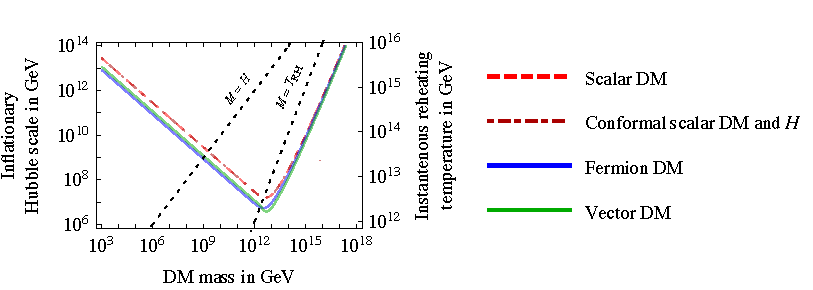
\includegraphics[width=0.9\textwidth]{figs/OmegaGravitationalDM} $$
\caption[Gravitational Dark Matter]{\label{fig:GravitationalDM}\em Curves along which freeze-in thermal production
of {\bfseries DM with gravitational couplings} reproduces the DM abundance. 
The dashed black lines indicate at which values the DM mass $M$ equals either the reheating temperature $T_{\rm RH}$
or the inflationary Hubble constant.}
\end{figure}



\section{Gravitational Dark Matter}\label{GravDM}
\index{Gravitational DM}\index{DM cosmological abundance!gravitational}\index{DM theory!gravitational}
So far, we only observed gravitational interactions of DM.
One can thereby consider theories where DM is a particle (a singlet scalar $S$, a singlet fermion $N$, or a massive vector $V$) endowed with only gravitational interactions~\cite{GravDM}.
The graviton interactions with matter are theoretically well known: 
expanding $g_{\mu\nu} = \eta_{\mu\nu} + 2 h_{\mu\nu}/\bar{M}_{\rm Pl}$,
the interaction of a single graviton is $\Lag_{\rm int}=h_{\mu\nu} T^{\mu\nu}/\bar{M}_{\rm Pl}$,
where $T_{\mu\nu}$ is the energy-momentum tensor  whose form depends on whether DM is a scalar, a fermion or a vector. 
At sub-Planckian energies graviton exchanges result in power suppressed interactions, with the effective coupling given by $g_{\rm grav} \sim E/M_{\rm Pl}$.
For scalar DM the gravitational interactions  also contain an additional non-minimal coupling, $\xi_S\,  RS^2/2$, where $R$ is the Ricci scalar, 
and $\xi_S$ is a dimensionless coupling. Below, we will mostly be able to ignore the effects of this non-minimal coupling, while  it needs to be taken into account for more detailed results. 

In the early Universe, there are two main mechanisms for production of particles with only gravitational interactions:  
either through  freeze-in during the thermal phase of cosmology (section~\ref{Freeze-in}),
or already earlier, during inflation (section~\ref{sec:inflDMprod}).
 \begin{itemize}
\item[\scalebox{0.6}{$\blacksquare$}] {\bf Freeze-in}. The amplitude for the SM SM $\to$ DM DM scatterings mediated by the $s$-wave graviton exchange is, at energies
much above the SM particle masses, given by
$\mathscr{A}= -i  \sfrac{T_{\mu\nu} T^{\mu\nu}}{\bar{M}_{\rm Pl}^2 s}$, where $s$ is the center of mass energy squared. The resulting predictions for the scattering cross sections, including $\mathcal{O}(1)$ factors, can be found in~\cite{GravDM}, while here we focus on the simple scaling estimates.  
The space-time density of scatterings that produce DM from the SM plasma
is $\gamma \sim T^8 e^{-2 M/T}/M_{\rm Pl}^4$ (with an 
additional $T/M$ $p$-wave suppression in the case of fermionic DM, which we ignore in the estimates below).
The resulting DM  number abundance is
\beq 
\label{eq:YDM:gravitational:freeze-in}
Y_{\rm DM} \approx \left.\frac{\gamma}{H s}\right|_{T =T_{\rm RH}}  \sim e^{-2 M/T_{\rm RH}} \left(\frac{T_{\rm RH}}{M_{\rm Pl}}\right)^3,
\eeq
where the reheating temperature is given by $T_{\rm RH} \sim\sqrt{M_{\rm Pl}H_{\rm infl}}$, if the reheating after the end of inflation
is instantaneous, while  $T_{\rm RH} \sim\sqrt{M_{\rm Pl}\Gamma_{\rm infl}}$ otherwise.
For any given $T_{\rm RH}$ the DM mass abundance, $\Omega_{\rm DM} \sim Y_{\rm DM} M/T_0$, is maximised for DM mass that is comparable to the reheat temperature, $M \sim T_{\rm RH}$, 
since this maximises the gravitational coupling while avoiding
the exponential suppression in eq.~\eqref{eq:YDM:gravitational:freeze-in}. The resulting
$\Omega_{\rm DM}^{\rm max} \sim M^4/M_{\rm Pl}^3 T_0$ matches
the observed DM density for $T_{\rm RH}\approx M \sim 10^{12}\GeV$. This is the minimal viable reheating temperature for gravitational DM; 
for lower $T_{\rm RH}$ the observed DM density cannot be reproduced.
For larger $T_{\rm RH}$ the observed DM density is matched for two values of DM mass, 
$M_{\rm heavier} \approx \hbox{few} \times T_{\rm RH}$, and $M_{\rm lighter}\approx (10^{12}\GeV)^4/T_{\rm RH}^3$, see fig.\fig{GravitationalDM}.



\item[\scalebox{0.6}{$\blacksquare$}] {\bf Inflation}. As we saw above, the freeze-in production of gravitational DM is dominated by the highest temperatures after the end of inflation. It is possible that an even larger effect arises during the preceding inflationary phase.
As discussed in section~\ref{sec:inflDMprod},
this includes two possibly dominant contributions that depend on the particular (unknown)  model of inflation, and occur in the final phases of the inflationary epoch:
the decay of the inflaton $\phi$ after  the end of inflation (DM production is kinematically blocked if $m_\phi < 2M$),
and the inflaton oscillations toward the end of inflation (kinematically blocked if $m_\phi\circa{<}M$).
The production of DM during the period of inflation itself, on the other hand, is less model-dependent, see section~\ref{sec:inflfluc}.
The end result, at least for $M \sim H_{\rm infl}$, is  DM with roughly thermal distribution corresponding to $T \approx H_{\rm infl}/2\pi$, and thereby a DM abundance $n \sim M^3 e^{-M/H_{\rm infl}}$, but the details are rather complicated. 
Importantly, the inflationary contribution to DM relic density can lead to problematic iso-curvature density fluctuations.
However, in the case of instantaneous reheating, the inflationary contribution is negligible compared to the freeze-in contribution, and can thus  safely be ignored.

\end{itemize}
From a theoretical point of view, the hypothesis that the DM particle only has gravitational interactions is quite intriguing.\footnote{Historically, one of the first proposals are {\em WIMPzillas}, introduced in section~\ref{ultraheavy}.} 
A priori, there is no good reason to forbid interactions such as the scalar DM quartic $|H|^2 |S|^2$, coupling $S$ to the Higgs boson, or a Yukawa interaction $LHN$ in the case of fermion DM $N$, or a mixing of a vector DM with the SM hypercharge gauge field, $B_\mu$.
Furthermore, if the mass of the vector DM is due to a Higgs mechanism, i.e., due the vacuum expectation value of a new dark scalar, $\varphi_{\rm dark}$,
the vector DM would also inherit any non-gravitational couplings of the dark scalar (in particular, there would be interactions between $\varphi_{\rm dark}$ and $V$).
The gravitational DM hypothesis posits that  all these, otherwise completely allowed renormalizable interactions, are for some reason highly suppressed to a sub-gravitational level.
Furthermore, it is not enough to forbid renormalizable interactions. Non-renormalizable Planck-suppressed operators that involve DM and SM particles, such as $S^2 \bar q q/M_{\rm Pl}$, naively give contributions that are comparable to the graviton mediated scatterings. Such operators are unavoidably generated by the quantum effects at the loop level. While they are loop suppressed, they are also logarithmically enhanced due to renormalisation group running from Planck scale to the energy scale at which scattering occurs, and can thus compete with gravitational interactions. 
In general, we can also expect that such operators are generated at tree level at the Planck scale
by the still poorly understood quantum gravity physics.

\smallskip

This does not mean that it is not possible to forbid the non-gravitational interactions via a symmetry. 
A particularly simple example is a dark sector that consists of just the gauge fields of
 a non-abelian `dark color' group $\mathcal{G}$~\cite{GravDM}, without any additional matter content. 
This gives rise to gravitationally-interacting (meta-)stable dark glue-balls, as discussed in section \ref{sec:darkglueballs}.
According to the conjectured AdS/CFT correspondence some of these theories admit a dual description:
special strong gauge dynamics with slowly running gauge coupling is equivalent to gravity in a warped extra dimension,
and glue-balls are equivalent to Kaluza-Klein excitations of gravitons.

This suggests that the lightest Kaluza-Klein excitation of a graviton propagating in generic extra dimensions (not necessarily warped)
can be one more candidate for gravitational DM.
It can be stable for special geometries, such as a flat segment with an orbifold reflection symmetry, with
the SM fields confined on a three dimensional boundary (see, e.g., \arxivref{1709.09688}{Garny et al.~(2017)} in~\cite{GravDM}). 
For further discussion of other realizations of DM in extra-dimensional set-ups 
see section~\ref{sec:swampDM} for connections with string theory, and section~\ref{sec:Xdim}  for connections with the hierarchy problem. 
The supersymmetric gravitino, to be discussed in section~\ref{sec:gravitinoDM}, can also behave as a gravitational DM, in a particular limit.

\medskip

DM particles with only gravitational interactions are very hard to search for directly (sometimes also referred as the {\em nightmare scenario}). 
Two exceptions arise in corners of the parameter space:
{\em i)} gravitational DM with  Planck-scale mass, which can be searched for in the laboratory using an array of mechanical sensors, see section~\ref{gravisignal};
{\em ii)} `large' extra dimensions with low quantum gravity scale comparable to the energy reached by colliders would allow, for instance, to produce
KK excitations of gravitons and extra dimensional black holes.
In addition, the {\sc Pao} collaboration derived constraints for the case of gravitational DM particles being able to decay into the SM particle via the non-perturbative effects due to a dark gauge group \cite{GravDM}.




